% Options for packages loaded elsewhere
\PassOptionsToPackage{unicode}{hyperref}
\PassOptionsToPackage{hyphens}{url}
%
\documentclass[
]{book}
\title{Sesión 1}
\author{Björn Reu, Yovanny Duran, Zarith Villamizar, Silvia Ardila y Sergio Bolivar}
\date{2021-11-05}

\usepackage{amsmath,amssymb}
\usepackage{lmodern}
\usepackage{iftex}
\ifPDFTeX
  \usepackage[T1]{fontenc}
  \usepackage[utf8]{inputenc}
  \usepackage{textcomp} % provide euro and other symbols
\else % if luatex or xetex
  \usepackage{unicode-math}
  \defaultfontfeatures{Scale=MatchLowercase}
  \defaultfontfeatures[\rmfamily]{Ligatures=TeX,Scale=1}
\fi
% Use upquote if available, for straight quotes in verbatim environments
\IfFileExists{upquote.sty}{\usepackage{upquote}}{}
\IfFileExists{microtype.sty}{% use microtype if available
  \usepackage[]{microtype}
  \UseMicrotypeSet[protrusion]{basicmath} % disable protrusion for tt fonts
}{}
\makeatletter
\@ifundefined{KOMAClassName}{% if non-KOMA class
  \IfFileExists{parskip.sty}{%
    \usepackage{parskip}
  }{% else
    \setlength{\parindent}{0pt}
    \setlength{\parskip}{6pt plus 2pt minus 1pt}}
}{% if KOMA class
  \KOMAoptions{parskip=half}}
\makeatother
\usepackage{xcolor}
\IfFileExists{xurl.sty}{\usepackage{xurl}}{} % add URL line breaks if available
\IfFileExists{bookmark.sty}{\usepackage{bookmark}}{\usepackage{hyperref}}
\hypersetup{
  pdftitle={Sesión 1},
  pdfauthor={Björn Reu, Yovanny Duran, Zarith Villamizar, Silvia Ardila y Sergio Bolivar},
  hidelinks,
  pdfcreator={LaTeX via pandoc}}
\urlstyle{same} % disable monospaced font for URLs
\usepackage{color}
\usepackage{fancyvrb}
\newcommand{\VerbBar}{|}
\newcommand{\VERB}{\Verb[commandchars=\\\{\}]}
\DefineVerbatimEnvironment{Highlighting}{Verbatim}{commandchars=\\\{\}}
% Add ',fontsize=\small' for more characters per line
\usepackage{framed}
\definecolor{shadecolor}{RGB}{248,248,248}
\newenvironment{Shaded}{\begin{snugshade}}{\end{snugshade}}
\newcommand{\AlertTok}[1]{\textcolor[rgb]{0.94,0.16,0.16}{#1}}
\newcommand{\AnnotationTok}[1]{\textcolor[rgb]{0.56,0.35,0.01}{\textbf{\textit{#1}}}}
\newcommand{\AttributeTok}[1]{\textcolor[rgb]{0.77,0.63,0.00}{#1}}
\newcommand{\BaseNTok}[1]{\textcolor[rgb]{0.00,0.00,0.81}{#1}}
\newcommand{\BuiltInTok}[1]{#1}
\newcommand{\CharTok}[1]{\textcolor[rgb]{0.31,0.60,0.02}{#1}}
\newcommand{\CommentTok}[1]{\textcolor[rgb]{0.56,0.35,0.01}{\textit{#1}}}
\newcommand{\CommentVarTok}[1]{\textcolor[rgb]{0.56,0.35,0.01}{\textbf{\textit{#1}}}}
\newcommand{\ConstantTok}[1]{\textcolor[rgb]{0.00,0.00,0.00}{#1}}
\newcommand{\ControlFlowTok}[1]{\textcolor[rgb]{0.13,0.29,0.53}{\textbf{#1}}}
\newcommand{\DataTypeTok}[1]{\textcolor[rgb]{0.13,0.29,0.53}{#1}}
\newcommand{\DecValTok}[1]{\textcolor[rgb]{0.00,0.00,0.81}{#1}}
\newcommand{\DocumentationTok}[1]{\textcolor[rgb]{0.56,0.35,0.01}{\textbf{\textit{#1}}}}
\newcommand{\ErrorTok}[1]{\textcolor[rgb]{0.64,0.00,0.00}{\textbf{#1}}}
\newcommand{\ExtensionTok}[1]{#1}
\newcommand{\FloatTok}[1]{\textcolor[rgb]{0.00,0.00,0.81}{#1}}
\newcommand{\FunctionTok}[1]{\textcolor[rgb]{0.00,0.00,0.00}{#1}}
\newcommand{\ImportTok}[1]{#1}
\newcommand{\InformationTok}[1]{\textcolor[rgb]{0.56,0.35,0.01}{\textbf{\textit{#1}}}}
\newcommand{\KeywordTok}[1]{\textcolor[rgb]{0.13,0.29,0.53}{\textbf{#1}}}
\newcommand{\NormalTok}[1]{#1}
\newcommand{\OperatorTok}[1]{\textcolor[rgb]{0.81,0.36,0.00}{\textbf{#1}}}
\newcommand{\OtherTok}[1]{\textcolor[rgb]{0.56,0.35,0.01}{#1}}
\newcommand{\PreprocessorTok}[1]{\textcolor[rgb]{0.56,0.35,0.01}{\textit{#1}}}
\newcommand{\RegionMarkerTok}[1]{#1}
\newcommand{\SpecialCharTok}[1]{\textcolor[rgb]{0.00,0.00,0.00}{#1}}
\newcommand{\SpecialStringTok}[1]{\textcolor[rgb]{0.31,0.60,0.02}{#1}}
\newcommand{\StringTok}[1]{\textcolor[rgb]{0.31,0.60,0.02}{#1}}
\newcommand{\VariableTok}[1]{\textcolor[rgb]{0.00,0.00,0.00}{#1}}
\newcommand{\VerbatimStringTok}[1]{\textcolor[rgb]{0.31,0.60,0.02}{#1}}
\newcommand{\WarningTok}[1]{\textcolor[rgb]{0.56,0.35,0.01}{\textbf{\textit{#1}}}}
\usepackage{longtable,booktabs,array}
\usepackage{calc} % for calculating minipage widths
% Correct order of tables after \paragraph or \subparagraph
\usepackage{etoolbox}
\makeatletter
\patchcmd\longtable{\par}{\if@noskipsec\mbox{}\fi\par}{}{}
\makeatother
% Allow footnotes in longtable head/foot
\IfFileExists{footnotehyper.sty}{\usepackage{footnotehyper}}{\usepackage{footnote}}
\makesavenoteenv{longtable}
\usepackage{graphicx}
\makeatletter
\def\maxwidth{\ifdim\Gin@nat@width>\linewidth\linewidth\else\Gin@nat@width\fi}
\def\maxheight{\ifdim\Gin@nat@height>\textheight\textheight\else\Gin@nat@height\fi}
\makeatother
% Scale images if necessary, so that they will not overflow the page
% margins by default, and it is still possible to overwrite the defaults
% using explicit options in \includegraphics[width, height, ...]{}
\setkeys{Gin}{width=\maxwidth,height=\maxheight,keepaspectratio}
% Set default figure placement to htbp
\makeatletter
\def\fps@figure{htbp}
\makeatother
\setlength{\emergencystretch}{3em} % prevent overfull lines
\providecommand{\tightlist}{%
  \setlength{\itemsep}{0pt}\setlength{\parskip}{0pt}}
\setcounter{secnumdepth}{5}
\usepackage{booktabs}
\ifLuaTeX
  \usepackage{selnolig}  % disable illegal ligatures
\fi
\usepackage[]{natbib}
\bibliographystyle{apalike}

\begin{document}
\maketitle

{
\setcounter{tocdepth}{1}
\tableofcontents
}
\hypertarget{preface}{%
\chapter*{Preface}\label{preface}}
\addcontentsline{toc}{chapter}{Preface}

This is the very first part of the book.

\hypertarget{introducciuxf3n}{%
\chapter{Introducción}\label{introducciuxf3n}}

El curso Introducción al análisis de datos utilizando R está dirigido a estudiantes de Biología y de Ingeniería Forestal en sus primeros semestres para familiarizarlos con el uso del lenguaje de programación R.

R es un lenguaje de programación de entorno de software libre para computación estadística y gráfica (R Development Core Team, 2021). En años recientes, R se ha vuelto una herramienta indispensable para el análisis de datos (o ciencia de datos) en muchas áreas de las ciencias básicas y aplicadas (Tippmann, 2015) y en la industria (Gandrud, 2013). En lugar de aprender múltiples herramientas, los estudiantes pueden utilizar un entorno único para una gran diversidad de métodos de análisis de datos. Más que un lenguaje de programación, R ofrece nuevas vías para la enseñanza de la estadística y análisis de datos, debido a que los problemas estadísticos pueden ser desarrollados y analizados de manera transparente y reproducible (Incerti et al., 2019). Esto permite un aprendizaje interactivo y orientado a resolver problemas, combinando la teoría y la práctica. De esta manera, los estudiantes pueden lograr una comprensión más profunda de análisis de datos de forma más sencilla, lo cual les permitirá practicar análisis de datos durante sus estudios utilizando todas las herramientas y posibilidades que les ofrece el lenguaje de programación R.

Este libro y el diseño del curso Introducción al análisis de datos utilizando R son el resultado del proyecto Análisis de datos utilizando el lenguaje de programación R: una experiencia de aprendizaje virtual en el aula invertida, de la convocatoría Iniciativas de innovación didáctica mediante el uso de tecnologías, INNOVA-TIC 2021 de la Vicerrectoría Académica de la Universidad Industrial de Santander, UIS.

\hypertarget{introducciuxf3n-a-la-programaciuxf3n-con-r}{%
\chapter{Introducción a la programación con R}\label{introducciuxf3n-a-la-programaciuxf3n-con-r}}

Comenzaremos con las operaciones básicas ejecutadas en la línea de comandos en R o terminal. Este será nuestro espacio de trabajo en el cual ejecutaremos las ordenes cuyos resultados se mostrarán en la consola.

Todo lo que siga después de un numeral (\#) será considerado como un comentario que al ejecutar será omitido. Para ejecutar el código en R podemos utilizar el botón ``run'' que disponemos arriba a la derecha, o utilizar un atajo:

\begin{itemize}
\tightlist
\item
  \textbf{Command + Enter (Mac)}
\item
  \textbf{Control + Enter (Windows, Linux)}
\end{itemize}

\hypertarget{la-luxednea-de-comandos-terminal}{%
\subsection{La línea de comandos (Terminal)}\label{la-luxednea-de-comandos-terminal}}

Línea de comandos como calculadora:

\begin{Shaded}
\begin{Highlighting}[]
\DecValTok{2}\SpecialCharTok{+}\DecValTok{5}
\SpecialCharTok{{-}}\NormalTok{ [}\DecValTok{1}\NormalTok{] }\DecValTok{7}
\DecValTok{7{-}3}
\SpecialCharTok{{-}}\NormalTok{ [}\DecValTok{1}\NormalTok{] }\DecValTok{4}
\NormalTok{(}\DecValTok{2}\SpecialCharTok{+}\DecValTok{3}\NormalTok{)}\SpecialCharTok{*}\DecValTok{5}
\SpecialCharTok{{-}}\NormalTok{ [}\DecValTok{1}\NormalTok{] }\DecValTok{25}
\NormalTok{(}\DecValTok{2}\SpecialCharTok{+}\DecValTok{3}\NormalTok{)}\SpecialCharTok{/}\NormalTok{((}\DecValTok{2}\SpecialCharTok{+}\DecValTok{3}\NormalTok{)}\SpecialCharTok{*}\DecValTok{5}\NormalTok{)}
\SpecialCharTok{{-}}\NormalTok{ [}\DecValTok{1}\NormalTok{] }\FloatTok{0.2}
\end{Highlighting}
\end{Shaded}

Se pueden ejecutar varias operaciones utilizando punto y coma (;):

\begin{Shaded}
\begin{Highlighting}[]
\DecValTok{2}\SpecialCharTok{+}\DecValTok{5}\NormalTok{; }\DecValTok{4}\SpecialCharTok{+}\DecValTok{6}
\SpecialCharTok{{-}}\NormalTok{ [}\DecValTok{1}\NormalTok{] }\DecValTok{7}
\SpecialCharTok{{-}}\NormalTok{ [}\DecValTok{1}\NormalTok{] }\DecValTok{10}
\end{Highlighting}
\end{Shaded}

Dispone de diferentes funciones como raíz cuadrada o logaritmo:

\begin{Shaded}
\begin{Highlighting}[]
\NormalTok{?Arithmetic}
\SpecialCharTok{{-}}\NormalTok{ starting httpd help server ... done}
\FunctionTok{sqrt}\NormalTok{(}\DecValTok{9}\NormalTok{) }\CommentTok{\# *raíz cuadrada*}
\SpecialCharTok{{-}}\NormalTok{ [}\DecValTok{1}\NormalTok{] }\DecValTok{3}
\FunctionTok{log}\NormalTok{(}\DecValTok{1}\NormalTok{)  }\CommentTok{\# logaritmo}
\SpecialCharTok{{-}}\NormalTok{ [}\DecValTok{1}\NormalTok{] }\DecValTok{0}
\FunctionTok{log10}\NormalTok{(}\DecValTok{10}\NormalTok{) }\CommentTok{\# logaritmo base 10}
\SpecialCharTok{{-}}\NormalTok{ [}\DecValTok{1}\NormalTok{] }\DecValTok{1}
\DecValTok{3}\SpecialCharTok{\^{}}\DecValTok{2} \CommentTok{\# potenciación (exponente 2)}
\SpecialCharTok{{-}}\NormalTok{ [}\DecValTok{1}\NormalTok{] }\DecValTok{9}
\end{Highlighting}
\end{Shaded}

Las letras y variables más importantes estan disponibles en R:

\begin{Shaded}
\begin{Highlighting}[]
\NormalTok{?Constants}
\NormalTok{pi}
\SpecialCharTok{{-}}\NormalTok{ [}\DecValTok{1}\NormalTok{] }\FloatTok{3.141593}
\NormalTok{letters}
\SpecialCharTok{{-}}\NormalTok{  [}\DecValTok{1}\NormalTok{] }\StringTok{"a"} \StringTok{"b"} \StringTok{"c"} \StringTok{"d"} \StringTok{"e"} \StringTok{"f"} \StringTok{"g"} \StringTok{"h"} \StringTok{"i"} \StringTok{"j"} \StringTok{"k"} \StringTok{"l"} \StringTok{"m"} \StringTok{"n"} \StringTok{"o"} \StringTok{"p"} \StringTok{"q"} \StringTok{"r"} \StringTok{"s"}
\SpecialCharTok{{-}}\NormalTok{ [}\DecValTok{20}\NormalTok{] }\StringTok{"t"} \StringTok{"u"} \StringTok{"v"} \StringTok{"w"} \StringTok{"x"} \StringTok{"y"} \StringTok{"z"}
\NormalTok{LETTERS}
\SpecialCharTok{{-}}\NormalTok{  [}\DecValTok{1}\NormalTok{] }\StringTok{"A"} \StringTok{"B"} \StringTok{"C"} \StringTok{"D"} \StringTok{"E"} \StringTok{"F"} \StringTok{"G"} \StringTok{"H"} \StringTok{"I"} \StringTok{"J"} \StringTok{"K"} \StringTok{"L"} \StringTok{"M"} \StringTok{"N"} \StringTok{"O"} \StringTok{"P"} \StringTok{"Q"} \StringTok{"R"} \StringTok{"S"}
\SpecialCharTok{{-}}\NormalTok{ [}\DecValTok{20}\NormalTok{] }\StringTok{"T"} \StringTok{"U"} \StringTok{"V"} \StringTok{"W"} \StringTok{"X"} \StringTok{"Y"} \StringTok{"Z"}
\end{Highlighting}
\end{Shaded}

\begin{center}\rule{0.5\linewidth}{0.5pt}\end{center}

\hypertarget{funciuxf3n-ayuda}{%
\subsection{Función ayuda}\label{funciuxf3n-ayuda}}

Existen tres formas de obtener ayuda:

\begin{itemize}
\tightlist
\item
  Área miscelánea -\textgreater{} ``Help''
\item
  Símbolo ``?'' antes de la función
\item
  Tecla Tabulador (Autocompleta el nombre)
\end{itemize}

\begin{Shaded}
\begin{Highlighting}[]
\NormalTok{x }\OtherTok{\textless{}{-}} \FunctionTok{c}\NormalTok{(}\DecValTok{1}\NormalTok{,}\DecValTok{2}\NormalTok{,}\DecValTok{3}\NormalTok{,}\DecValTok{4}\NormalTok{,}\DecValTok{5}\NormalTok{,}\DecValTok{6}\NormalTok{,}\DecValTok{7}\NormalTok{,}\DecValTok{8}\NormalTok{) }\CommentTok{\# \textless{}{-} símbolo de asignación, permite agrupar los elementos dentro del objeto }
\end{Highlighting}
\end{Shaded}

\begin{Shaded}
\begin{Highlighting}[]
\NormalTok{x }\OtherTok{=} \FunctionTok{c}\NormalTok{(}\DecValTok{1}\NormalTok{,}\DecValTok{2}\NormalTok{,}\DecValTok{3}\NormalTok{,}\DecValTok{4}\NormalTok{,}\DecValTok{5}\NormalTok{,}\DecValTok{6}\NormalTok{,}\DecValTok{7}\NormalTok{,}\DecValTok{8}\NormalTok{) }\CommentTok{\# "\textless{}{-}" o "=" significa lo mismo}
\end{Highlighting}
\end{Shaded}

\begin{Shaded}
\begin{Highlighting}[]
\FunctionTok{mean}\NormalTok{(x)}
\SpecialCharTok{{-}}\NormalTok{ [}\DecValTok{1}\NormalTok{] }\FloatTok{4.5}
\NormalTok{?sum}
\NormalTok{?rep}
\NormalTok{?sort}
\NormalTok{?order}
\end{Highlighting}
\end{Shaded}

Estructura de la función:

\begin{itemize}
\tightlist
\item
  Función: ``mean()''
\item
  Objeto: ``x''
\item
  Argumento (`arg'): ``na.rm=FALSE''
\end{itemize}

\begin{quote}
\textbf{Ejercicio 1:}
\end{quote}

\begin{itemize}
\tightlist
\item
  \emph{Explicar brevemente la función ``order''. ¿Qué hace y qué significan los argumentos?}
\end{itemize}

\begin{center}\rule{0.5\linewidth}{0.5pt}\end{center}

\hypertarget{creando-nuevas-variables}{%
\subsection{Creando nuevas variables:}\label{creando-nuevas-variables}}

Para crear una nueva variable usted puede utilizar ``\textless-'' (símbolo de asignación) o ``=''. Es aconsejable el uso de ``\textless-'' ya que se refiere a la indexación dentro de un vector.

Cada variable necesita un nombre que puede estar compuesto de letras, números, ``.'' o ``\_'' y nunca por números. Ejemplo: ``my\_data''.

R diferencia entre minúsculas y mayúsculas; ``a'' es diferente de ``A''. Las variables pueden ser reescritas. Una vez escrita una variable podemos llamar al objeto:

\begin{Shaded}
\begin{Highlighting}[]
\NormalTok{x }\OtherTok{\textless{}{-}} \DecValTok{3}
\NormalTok{x}
\SpecialCharTok{{-}}\NormalTok{ [}\DecValTok{1}\NormalTok{] }\DecValTok{3}
\NormalTok{x }\OtherTok{\textless{}{-}} \DecValTok{9}
\NormalTok{x}
\SpecialCharTok{{-}}\NormalTok{ [}\DecValTok{1}\NormalTok{] }\DecValTok{9}
\NormalTok{resultado }\OtherTok{\textless{}{-}} \DecValTok{3}\SpecialCharTok{+}\DecValTok{9}
\NormalTok{resultado}
\SpecialCharTok{{-}}\NormalTok{ [}\DecValTok{1}\NormalTok{] }\DecValTok{12}
\FunctionTok{mode}\NormalTok{(resultado)}
\SpecialCharTok{{-}}\NormalTok{ [}\DecValTok{1}\NormalTok{] }\StringTok{"numeric"}
\end{Highlighting}
\end{Shaded}

Además de las variables (`numeric'), R permite la definición de texto (`character') y de variables lógicas (`logic', ej: TRUE y FALSE). Los caracteres deben ser puestos entre comillas dobles (``\ldots{}'') para que R los identifique como tal.

Estos tipos de vectores se definen como vectores atómicos:

\begin{Shaded}
\begin{Highlighting}[]
\NormalTok{y }\OtherTok{\textless{}{-}} \StringTok{"test"}
\NormalTok{y}
\SpecialCharTok{{-}}\NormalTok{ [}\DecValTok{1}\NormalTok{] }\StringTok{"test"}
\FunctionTok{mode}\NormalTok{(y)}
\SpecialCharTok{{-}}\NormalTok{ [}\DecValTok{1}\NormalTok{] }\StringTok{"character"}
\NormalTok{a }\OtherTok{\textless{}{-}} \ConstantTok{FALSE}
\NormalTok{a}
\SpecialCharTok{{-}}\NormalTok{ [}\DecValTok{1}\NormalTok{] }\ConstantTok{FALSE}
\FunctionTok{mode}\NormalTok{(a)}
\SpecialCharTok{{-}}\NormalTok{ [}\DecValTok{1}\NormalTok{] }\StringTok{"logical"}
\FunctionTok{mode}\NormalTok{(T) }\CommentTok{\# T es igual a TRUE, y F es igual a FALSE}
\SpecialCharTok{{-}}\NormalTok{ [}\DecValTok{1}\NormalTok{] }\StringTok{"logical"}
\end{Highlighting}
\end{Shaded}

¿Qué ocurre aquí?

\begin{Shaded}
\begin{Highlighting}[]
\NormalTok{s }\OtherTok{\textless{}{-}} \FunctionTok{as.numeric}\NormalTok{(}\FunctionTok{c}\NormalTok{(T,F,F)) }
\FunctionTok{mode}\NormalTok{(s)}
\SpecialCharTok{{-}}\NormalTok{ [}\DecValTok{1}\NormalTok{] }\StringTok{"numeric"}
\end{Highlighting}
\end{Shaded}

\begin{center}\rule{0.5\linewidth}{0.5pt}\end{center}

\hypertarget{el-uxe1rea-de-trabajo-o-memoria---ventana-arriba-a-la-derecha-environment}{%
\subsection{El área de trabajo o memoria - Ventana arriba a la derecha `Environment'}\label{el-uxe1rea-de-trabajo-o-memoria---ventana-arriba-a-la-derecha-environment}}

Todos los objetos creados durante una sesión son guardados en el área de trabajo. Para ver el área de trabajo ejecute ls(), para remover algún objeto de esta ejecute rm().

También puede utilizar los botones en el área de trabajo

\begin{Shaded}
\begin{Highlighting}[]
\FunctionTok{ls}\NormalTok{()}
\SpecialCharTok{{-}}\NormalTok{ [}\DecValTok{1}\NormalTok{] }\StringTok{"a"}         \StringTok{"resultado"} \StringTok{"s"}         \StringTok{"x"}         \StringTok{"y"}
\FunctionTok{rm}\NormalTok{(s)}
\FunctionTok{ls}\NormalTok{()}
\SpecialCharTok{{-}}\NormalTok{ [}\DecValTok{1}\NormalTok{] }\StringTok{"a"}         \StringTok{"resultado"} \StringTok{"x"}         \StringTok{"y"}
\end{Highlighting}
\end{Shaded}

\begin{center}\rule{0.5\linewidth}{0.5pt}\end{center}

\hypertarget{vamos-a-practicar}{%
\subsection{Vamos a practicar}\label{vamos-a-practicar}}

Puedes hacer cálculos simples con variables númericas

\begin{Shaded}
\begin{Highlighting}[]
\NormalTok{a }\OtherTok{\textless{}{-}} \DecValTok{5}
\NormalTok{b }\OtherTok{\textless{}{-}} \DecValTok{7}
\NormalTok{a}\SpecialCharTok{+}\NormalTok{b}\SpecialCharTok{+}\DecValTok{3}
\SpecialCharTok{{-}}\NormalTok{ [}\DecValTok{1}\NormalTok{] }\DecValTok{15}
\end{Highlighting}
\end{Shaded}

¿Qué ocurre a continuación? Por favor explique.

\begin{Shaded}
\begin{Highlighting}[]
\NormalTok{b }\OtherTok{=} \DecValTok{2}
\NormalTok{b }\SpecialCharTok{==} \DecValTok{2}
\SpecialCharTok{{-}}\NormalTok{ [}\DecValTok{1}\NormalTok{] }\ConstantTok{TRUE}
\NormalTok{b }\SpecialCharTok{==} \DecValTok{3}
\SpecialCharTok{{-}}\NormalTok{ [}\DecValTok{1}\NormalTok{] }\ConstantTok{FALSE}
\NormalTok{c }\OtherTok{=} \DecValTok{7}
\NormalTok{d }\OtherTok{=} \SpecialCharTok{{-}}\DecValTok{3}
\NormalTok{?Syntax}
\end{Highlighting}
\end{Shaded}

\begin{quote}
\textbf{Ejercicio 2:}
\end{quote}

\begin{itemize}
\item
  \emph{Comprobar las siguientes afirmaciones lógicas:}

  \begin{itemize}
  \item
    ``c'' mayor que ``d''
  \item
    ``c'' menor o igual que ``d''
  \item
    ``c'' igual a ``d''
  \end{itemize}
\end{itemize}

\begin{center}\rule{0.5\linewidth}{0.5pt}\end{center}

\hypertarget{r-como-calculadora---operadores-y-funciones.}{%
\subsection{R como calculadora - Operadores y funciones.}\label{r-como-calculadora---operadores-y-funciones.}}

\begin{verbatim}
?Syntax

* <-               Asignar
* + - * / % ^      Aritméticas
* > >= < <= == !=  Relación (orden y comparación)
* ! & && | ||      lógicas
* $                lista indexada
* :                Crear una secuencia
\end{verbatim}

Operadores lógicos para:

\begin{verbatim}
* !      NO
* &      Y
* |      O
* <     Menor que
* <=    Menor o igual que
* >     Mayor que
* >=    Mayor o igual que
* ==    IGUAL
* !=    NO IGUAL (diferente de)
* &&    AND with IF (y con si <condicional>)
* ||    OR with IF (o con si <condicional>)
\end{verbatim}

\begin{center}\rule{0.5\linewidth}{0.5pt}\end{center}

\hypertarget{tipos-de-datos-y-objetos}{%
\subsection{Tipos de Datos y Objetos}\label{tipos-de-datos-y-objetos}}

\begin{itemize}
\tightlist
\item
  \textbf{``Logical''} :(FALSO/VERDADERO) / (FALSE/TRUE)
\item
  \textbf{``Number''} : (Entero, Decimal, Complejo (e.g.~3i))
\item
  \textbf{``Character''} : Letras y palabras (``\,``, o '\,')
\end{itemize}

Otros tipos de datos son \textbf{``list''}, \textbf{``expression''}, \textbf{``name''}, \textbf{``symbol''} and \textbf{``function''}

Para operaciones más complejas necesitamos estructuras de datos más complejas. R ofrece más que solo objetos que contienen un elemento, como los vectores o las matrices.

\begin{center}\rule{0.5\linewidth}{0.5pt}\end{center}

\hypertarget{vectores-i-vectores-sencillos}{%
\subsection{Vectores I: Vectores sencillos}\label{vectores-i-vectores-sencillos}}

Para hacer un vector utilice la función concatenar ``c()'' . Los elementos sencillos de un vector están separados por ``,''.

\begin{Shaded}
\begin{Highlighting}[]
\NormalTok{x }\OtherTok{\textless{}{-}} \FunctionTok{c}\NormalTok{ (}\DecValTok{2}\NormalTok{, }\DecValTok{5}\NormalTok{, }\DecValTok{10}\NormalTok{, }\DecValTok{14}\NormalTok{, }\DecValTok{3}\NormalTok{, }\DecValTok{1}\NormalTok{, }\DecValTok{18}\NormalTok{, }\DecValTok{24}\NormalTok{, }\DecValTok{17}\NormalTok{)}
\NormalTok{x}
\SpecialCharTok{{-}}\NormalTok{ [}\DecValTok{1}\NormalTok{]  }\DecValTok{2}  \DecValTok{5} \DecValTok{10} \DecValTok{14}  \DecValTok{3}  \DecValTok{1} \DecValTok{18} \DecValTok{24} \DecValTok{17}
\FunctionTok{mode}\NormalTok{(x)}
\SpecialCharTok{{-}}\NormalTok{ [}\DecValTok{1}\NormalTok{] }\StringTok{"numeric"}
\end{Highlighting}
\end{Shaded}

\begin{Shaded}
\begin{Highlighting}[]
\NormalTok{a }\OtherTok{\textless{}{-}} \FunctionTok{c}\NormalTok{ (}\StringTok{"text"}\NormalTok{, }\DecValTok{2}\NormalTok{, }\DecValTok{6}\NormalTok{, }\ConstantTok{TRUE}\NormalTok{)}
\FunctionTok{mode}\NormalTok{(a) }\DocumentationTok{\#\# ¿Qué ocurre aquí? Por qué "character"?}
\SpecialCharTok{{-}}\NormalTok{ [}\DecValTok{1}\NormalTok{] }\StringTok{"character"}
\NormalTok{a }\OtherTok{\textless{}{-}} \FunctionTok{c}\NormalTok{ ( }\DecValTok{2}\NormalTok{, }\DecValTok{6}\NormalTok{, F)}
\FunctionTok{mode}\NormalTok{(a) }\CommentTok{\#y ahora?}
\SpecialCharTok{{-}}\NormalTok{ [}\DecValTok{1}\NormalTok{] }\StringTok{"numeric"}
\end{Highlighting}
\end{Shaded}

Crear un vector vacío:

\begin{Shaded}
\begin{Highlighting}[]
\NormalTok{b }\OtherTok{\textless{}{-}} \FunctionTok{numeric}\NormalTok{(}\DecValTok{20}\NormalTok{)}
\NormalTok{b}
\SpecialCharTok{{-}}\NormalTok{  [}\DecValTok{1}\NormalTok{] }\DecValTok{0} \DecValTok{0} \DecValTok{0} \DecValTok{0} \DecValTok{0} \DecValTok{0} \DecValTok{0} \DecValTok{0} \DecValTok{0} \DecValTok{0} \DecValTok{0} \DecValTok{0} \DecValTok{0} \DecValTok{0} \DecValTok{0} \DecValTok{0} \DecValTok{0} \DecValTok{0} \DecValTok{0} \DecValTok{0}
\end{Highlighting}
\end{Shaded}

\begin{quote}
\textbf{Ejercicio 3:}
\end{quote}

\begin{itemize}
\tightlist
\item
  \emph{Crear un vector con nombre ``vec'' que contenga los números de 1 a 10.}
\end{itemize}

\begin{center}\rule{0.5\linewidth}{0.5pt}\end{center}

Un vector también puede contener diferentes tipos de variables. Usted puede realizar cálculos con vectores que contengan solo elementos ``numeric''

\begin{itemize}
\tightlist
\item
  \textbf{Suma}
\end{itemize}

\begin{Shaded}
\begin{Highlighting}[]
\FunctionTok{sort}\NormalTok{(x)}
\SpecialCharTok{{-}}\NormalTok{ [}\DecValTok{1}\NormalTok{]  }\DecValTok{1}  \DecValTok{2}  \DecValTok{3}  \DecValTok{5} \DecValTok{10} \DecValTok{14} \DecValTok{17} \DecValTok{18} \DecValTok{24}
\FunctionTok{sum}\NormalTok{(x)}
\SpecialCharTok{{-}}\NormalTok{ [}\DecValTok{1}\NormalTok{] }\DecValTok{94}
\end{Highlighting}
\end{Shaded}

\begin{itemize}
\tightlist
\item
  \textbf{Promedio}
\end{itemize}

\begin{Shaded}
\begin{Highlighting}[]
\FunctionTok{mean}\NormalTok{(x)}
\SpecialCharTok{{-}}\NormalTok{ [}\DecValTok{1}\NormalTok{] }\FloatTok{10.44444}
\end{Highlighting}
\end{Shaded}

\begin{itemize}
\tightlist
\item
  \textbf{Cuartil}
\end{itemize}

\begin{Shaded}
\begin{Highlighting}[]
\FunctionTok{quantile}\NormalTok{(x)}
\SpecialCharTok{{-}}   \DecValTok{0}\SpecialCharTok{\%  25\%}  \DecValTok{50}\SpecialCharTok{\%  75\%} \DecValTok{100}\NormalTok{\% }
\SpecialCharTok{{-}}    \DecValTok{1}    \DecValTok{3}   \DecValTok{10}   \DecValTok{17}   \DecValTok{24}
\end{Highlighting}
\end{Shaded}

\begin{itemize}
\tightlist
\item
  \textbf{Longitud del vector}
\end{itemize}

\begin{Shaded}
\begin{Highlighting}[]
\FunctionTok{length}\NormalTok{ (x)}
\SpecialCharTok{{-}}\NormalTok{ [}\DecValTok{1}\NormalTok{] }\DecValTok{9}
\FunctionTok{length}\NormalTok{(letters)}
\SpecialCharTok{{-}}\NormalTok{ [}\DecValTok{1}\NormalTok{] }\DecValTok{26}
\end{Highlighting}
\end{Shaded}

\begin{itemize}
\tightlist
\item
  \textbf{Ordenar}
\end{itemize}

\begin{Shaded}
\begin{Highlighting}[]
\NormalTok{x}
\SpecialCharTok{{-}}\NormalTok{ [}\DecValTok{1}\NormalTok{]  }\DecValTok{2}  \DecValTok{5} \DecValTok{10} \DecValTok{14}  \DecValTok{3}  \DecValTok{1} \DecValTok{18} \DecValTok{24} \DecValTok{17}
\NormalTok{?}\FunctionTok{sort}\NormalTok{(x)}
\FunctionTok{sort}\NormalTok{(x, }\AttributeTok{decreasing =}\NormalTok{ F)}
\SpecialCharTok{{-}}\NormalTok{ [}\DecValTok{1}\NormalTok{]  }\DecValTok{1}  \DecValTok{2}  \DecValTok{3}  \DecValTok{5} \DecValTok{10} \DecValTok{14} \DecValTok{17} \DecValTok{18} \DecValTok{24}
\FunctionTok{sort}\NormalTok{(x, }\AttributeTok{decreasing =} \ConstantTok{FALSE}\NormalTok{)}
\SpecialCharTok{{-}}\NormalTok{ [}\DecValTok{1}\NormalTok{]  }\DecValTok{1}  \DecValTok{2}  \DecValTok{3}  \DecValTok{5} \DecValTok{10} \DecValTok{14} \DecValTok{17} \DecValTok{18} \DecValTok{24}
\FunctionTok{sort}\NormalTok{(x, }\AttributeTok{decreasing =}\NormalTok{ T)}
\SpecialCharTok{{-}}\NormalTok{ [}\DecValTok{1}\NormalTok{] }\DecValTok{24} \DecValTok{18} \DecValTok{17} \DecValTok{14} \DecValTok{10}  \DecValTok{5}  \DecValTok{3}  \DecValTok{2}  \DecValTok{1}
\FunctionTok{sort}\NormalTok{(x, }\AttributeTok{decreasing =} \ConstantTok{TRUE}\NormalTok{)}
\SpecialCharTok{{-}}\NormalTok{ [}\DecValTok{1}\NormalTok{] }\DecValTok{24} \DecValTok{18} \DecValTok{17} \DecValTok{14} \DecValTok{10}  \DecValTok{5}  \DecValTok{3}  \DecValTok{2}  \DecValTok{1}
\end{Highlighting}
\end{Shaded}

¿Qué ocurre si colocamos ``decreasing = TRUE''? Compruebe con ``?sort''

\textbf{``sort''} y \textbf{``order''} realizan la misma función; sin embargo \textbf{``order''} puede ser aplicado a otro tipo de objetos diferentes a vectores, como los data frames.

\begin{itemize}
\tightlist
\item
  \textbf{Cálculo con vectores}
\end{itemize}

\begin{Shaded}
\begin{Highlighting}[]
\NormalTok{x}
\SpecialCharTok{{-}}\NormalTok{ [}\DecValTok{1}\NormalTok{]  }\DecValTok{2}  \DecValTok{5} \DecValTok{10} \DecValTok{14}  \DecValTok{3}  \DecValTok{1} \DecValTok{18} \DecValTok{24} \DecValTok{17}
\FunctionTok{length}\NormalTok{(x)}
\SpecialCharTok{{-}}\NormalTok{ [}\DecValTok{1}\NormalTok{] }\DecValTok{9}
\CommentTok{\#1}
\NormalTok{x }\SpecialCharTok{+} \DecValTok{10}
\SpecialCharTok{{-}}\NormalTok{ [}\DecValTok{1}\NormalTok{] }\DecValTok{12} \DecValTok{15} \DecValTok{20} \DecValTok{24} \DecValTok{13} \DecValTok{11} \DecValTok{28} \DecValTok{34} \DecValTok{27}
\NormalTok{x}
\SpecialCharTok{{-}}\NormalTok{ [}\DecValTok{1}\NormalTok{]  }\DecValTok{2}  \DecValTok{5} \DecValTok{10} \DecValTok{14}  \DecValTok{3}  \DecValTok{1} \DecValTok{18} \DecValTok{24} \DecValTok{17}
\CommentTok{\#2}
\NormalTok{y }\OtherTok{\textless{}{-}} \FunctionTok{c}\NormalTok{(}\DecValTok{1}\NormalTok{, }\DecValTok{3}\NormalTok{, }\DecValTok{5}\NormalTok{)}
\NormalTok{x }\SpecialCharTok{+}\NormalTok{ y}
\SpecialCharTok{{-}}\NormalTok{ [}\DecValTok{1}\NormalTok{]  }\DecValTok{3}  \DecValTok{8} \DecValTok{15} \DecValTok{15}  \DecValTok{6}  \DecValTok{6} \DecValTok{19} \DecValTok{27} \DecValTok{22}
\NormalTok{x}
\SpecialCharTok{{-}}\NormalTok{ [}\DecValTok{1}\NormalTok{]  }\DecValTok{2}  \DecValTok{5} \DecValTok{10} \DecValTok{14}  \DecValTok{3}  \DecValTok{1} \DecValTok{18} \DecValTok{24} \DecValTok{17}
\CommentTok{\#3}
\NormalTok{y }\OtherTok{\textless{}{-}} \FunctionTok{c}\NormalTok{ (}\DecValTok{4}\NormalTok{, }\DecValTok{2}\NormalTok{, }\DecValTok{8}\NormalTok{, }\DecValTok{5}\NormalTok{, }\DecValTok{3}\NormalTok{, }\DecValTok{9}\NormalTok{, }\DecValTok{3}\NormalTok{, }\DecValTok{10}\NormalTok{, }\DecValTok{1}\NormalTok{)}
\NormalTok{xy }\OtherTok{\textless{}{-}}\NormalTok{ x }\SpecialCharTok{+}\NormalTok{ y}
\NormalTok{xy}
\SpecialCharTok{{-}}\NormalTok{ [}\DecValTok{1}\NormalTok{]  }\DecValTok{6}  \DecValTok{7} \DecValTok{18} \DecValTok{19}  \DecValTok{6} \DecValTok{10} \DecValTok{21} \DecValTok{34} \DecValTok{18}
\NormalTok{x}
\SpecialCharTok{{-}}\NormalTok{ [}\DecValTok{1}\NormalTok{]  }\DecValTok{2}  \DecValTok{5} \DecValTok{10} \DecValTok{14}  \DecValTok{3}  \DecValTok{1} \DecValTok{18} \DecValTok{24} \DecValTok{17}
\CommentTok{\#4}
\NormalTok{y }\OtherTok{\textless{}{-}} \FunctionTok{c}\NormalTok{(}\DecValTok{1}\NormalTok{, }\DecValTok{3}\NormalTok{)}
\NormalTok{x }\SpecialCharTok{+}\NormalTok{ y}
\SpecialCharTok{{-}}\NormalTok{ Warning }\ControlFlowTok{in}\NormalTok{ x }\SpecialCharTok{+}\NormalTok{ y}\SpecialCharTok{:}\NormalTok{ longitud de objeto mayor no es múltiplo de la longitud de uno}
\SpecialCharTok{{-}}\NormalTok{ menor}
\SpecialCharTok{{-}}\NormalTok{ [}\DecValTok{1}\NormalTok{]  }\DecValTok{3}  \DecValTok{8} \DecValTok{11} \DecValTok{17}  \DecValTok{4}  \DecValTok{4} \DecValTok{19} \DecValTok{27} \DecValTok{18}
\NormalTok{x}
\SpecialCharTok{{-}}\NormalTok{ [}\DecValTok{1}\NormalTok{]  }\DecValTok{2}  \DecValTok{5} \DecValTok{10} \DecValTok{14}  \DecValTok{3}  \DecValTok{1} \DecValTok{18} \DecValTok{24} \DecValTok{17}
\CommentTok{\#5}
\NormalTok{y }\OtherTok{\textless{}{-}} \FunctionTok{c}\NormalTok{ (}\DecValTok{4}\NormalTok{, }\DecValTok{2}\NormalTok{, }\DecValTok{8}\NormalTok{, }\DecValTok{5}\NormalTok{, }\DecValTok{3}\NormalTok{, }\DecValTok{9}\NormalTok{, }\DecValTok{3}\NormalTok{, }\DecValTok{10}\NormalTok{, }\DecValTok{1}\NormalTok{)}
\FunctionTok{sum}\NormalTok{(x)}
\SpecialCharTok{{-}}\NormalTok{ [}\DecValTok{1}\NormalTok{] }\DecValTok{94}
\FunctionTok{sum}\NormalTok{(x,y)}
\SpecialCharTok{{-}}\NormalTok{ [}\DecValTok{1}\NormalTok{] }\DecValTok{139}
\FunctionTok{sum}\NormalTok{(x }\SpecialCharTok{+}\NormalTok{ y)}
\SpecialCharTok{{-}}\NormalTok{ [}\DecValTok{1}\NormalTok{] }\DecValTok{139}
\end{Highlighting}
\end{Shaded}

\begin{itemize}
\tightlist
\item
  \textbf{Etiquetas}
\end{itemize}

\begin{Shaded}
\begin{Highlighting}[]
\NormalTok{x }\OtherTok{\textless{}{-}} \FunctionTok{c}\NormalTok{ (}\DecValTok{2}\NormalTok{, }\DecValTok{5}\NormalTok{, }\DecValTok{10}\NormalTok{, }\DecValTok{14}\NormalTok{, }\DecValTok{3}\NormalTok{, }\DecValTok{1}\NormalTok{, }\DecValTok{18}\NormalTok{, }\DecValTok{24}\NormalTok{, }\DecValTok{17}\NormalTok{)}
\NormalTok{a }\OtherTok{\textless{}{-}} \FunctionTok{c}\NormalTok{ (}\StringTok{"E1"}\NormalTok{,}\StringTok{"E2"}\NormalTok{,}\StringTok{"E3"}\NormalTok{,}\StringTok{"E4"}\NormalTok{,}\StringTok{"E5"}\NormalTok{,}\StringTok{"E6"}\NormalTok{,}\StringTok{"E7"}\NormalTok{,}\StringTok{"E8"}\NormalTok{,}\StringTok{"E9"}\NormalTok{)}
\FunctionTok{names}\NormalTok{ (x) }\OtherTok{\textless{}{-}}\NormalTok{ a}
\NormalTok{x}
\SpecialCharTok{{-}}\NormalTok{ E1 E2 E3 E4 E5 E6 E7 E8 E9 }
\SpecialCharTok{{-}}  \DecValTok{2}  \DecValTok{5} \DecValTok{10} \DecValTok{14}  \DecValTok{3}  \DecValTok{1} \DecValTok{18} \DecValTok{24} \DecValTok{17}
\FunctionTok{names}\NormalTok{(x) }\CommentTok{\# Vector de los nombres del vector numérico x }
\SpecialCharTok{{-}}\NormalTok{ [}\DecValTok{1}\NormalTok{] }\StringTok{"E1"} \StringTok{"E2"} \StringTok{"E3"} \StringTok{"E4"} \StringTok{"E5"} \StringTok{"E6"} \StringTok{"E7"} \StringTok{"E8"} \StringTok{"E9"}
\FunctionTok{str}\NormalTok{ (x) }\CommentTok{\# sobre la estructura del vector x (muy útil!)}
\SpecialCharTok{{-}}\NormalTok{  Named num [}\DecValTok{1}\SpecialCharTok{:}\DecValTok{9}\NormalTok{] }\DecValTok{2} \DecValTok{5} \DecValTok{10} \DecValTok{14} \DecValTok{3} \DecValTok{1} \DecValTok{18} \DecValTok{24} \DecValTok{17}
\SpecialCharTok{{-}}  \SpecialCharTok{{-}} \FunctionTok{attr}\NormalTok{(}\SpecialCharTok{*}\NormalTok{, }\StringTok{"names"}\NormalTok{)}\OtherTok{=}\NormalTok{ chr [}\DecValTok{1}\SpecialCharTok{:}\DecValTok{9}\NormalTok{] }\StringTok{"E1"} \StringTok{"E2"} \StringTok{"E3"} \StringTok{"E4"}\NormalTok{ ...}
\FunctionTok{summary}\NormalTok{ (x) }\CommentTok{\# indica los valores mínimos, máximos, etc.}
\SpecialCharTok{{-}}\NormalTok{    Min. 1st Qu.  Median    Mean 3rd Qu.    Max. }
\SpecialCharTok{{-}}    \FloatTok{1.00}    \FloatTok{3.00}   \FloatTok{10.00}   \FloatTok{10.44}   \FloatTok{17.00}   \FloatTok{24.00}
\FunctionTok{head}\NormalTok{ (x)}
\SpecialCharTok{{-}}\NormalTok{ E1 E2 E3 E4 E5 E6 }
\SpecialCharTok{{-}}  \DecValTok{2}  \DecValTok{5} \DecValTok{10} \DecValTok{14}  \DecValTok{3}  \DecValTok{1}
\FunctionTok{tail}\NormalTok{ (x)}
\SpecialCharTok{{-}}\NormalTok{ E4 E5 E6 E7 E8 E9 }
\SpecialCharTok{{-}} \DecValTok{14}  \DecValTok{3}  \DecValTok{1} \DecValTok{18} \DecValTok{24} \DecValTok{17}
\end{Highlighting}
\end{Shaded}

\begin{quote}
\textbf{Ejercicio 4:}
\end{quote}

\begin{itemize}
\item
  \emph{Sumar los números enteros de 1 hasta 5.}
\item
  \emph{Crear un variable v1 que contenga una letra.}
\item
  \emph{Copiar v1 a v2.}
\item
  \emph{Comparar los valores de v1 y v2}
\item
  \emph{Crear un vector de longitud 20 con el tipo de datos que usted quiera y muestre las primeras nueve entradas.}
\item
  \emph{Crear un vector que contenga los seis primeras letras del abecedario.}
\end{itemize}

\begin{center}\rule{0.5\linewidth}{0.5pt}\end{center}

\hypertarget{vectores-ii-vectores-muxe1s-complejos}{%
\subsection{Vectores II: Vectores más complejos}\label{vectores-ii-vectores-muxe1s-complejos}}

\begin{itemize}
\tightlist
\item
  \textbf{Secuencias}
\end{itemize}

\begin{Shaded}
\begin{Highlighting}[]
\NormalTok{z }\OtherTok{\textless{}{-}} \DecValTok{3}\SpecialCharTok{:}\DecValTok{10}
\NormalTok{z}
\SpecialCharTok{{-}}\NormalTok{ [}\DecValTok{1}\NormalTok{]  }\DecValTok{3}  \DecValTok{4}  \DecValTok{5}  \DecValTok{6}  \DecValTok{7}  \DecValTok{8}  \DecValTok{9} \DecValTok{10}
\end{Highlighting}
\end{Shaded}

\begin{Shaded}
\begin{Highlighting}[]
\NormalTok{?seq}
\FunctionTok{seq}\NormalTok{(}\AttributeTok{from =} \DecValTok{1}\NormalTok{, }\AttributeTok{to =} \DecValTok{6}\NormalTok{, }\AttributeTok{by =} \FloatTok{0.2}\NormalTok{) }\CommentTok{\# El argumento "by" genera frecuencias \#}
\SpecialCharTok{{-}}\NormalTok{  [}\DecValTok{1}\NormalTok{] }\FloatTok{1.0} \FloatTok{1.2} \FloatTok{1.4} \FloatTok{1.6} \FloatTok{1.8} \FloatTok{2.0} \FloatTok{2.2} \FloatTok{2.4} \FloatTok{2.6} \FloatTok{2.8} \FloatTok{3.0} \FloatTok{3.2} \FloatTok{3.4} \FloatTok{3.6} \FloatTok{3.8} \FloatTok{4.0} \FloatTok{4.2} \FloatTok{4.4} \FloatTok{4.6}
\SpecialCharTok{{-}}\NormalTok{ [}\DecValTok{20}\NormalTok{] }\FloatTok{4.8} \FloatTok{5.0} \FloatTok{5.2} \FloatTok{5.4} \FloatTok{5.6} \FloatTok{5.8} \FloatTok{6.0}
\FunctionTok{seq}\NormalTok{(}\AttributeTok{from =} \DecValTok{1}\NormalTok{, }\AttributeTok{to =} \DecValTok{6}\NormalTok{, }\AttributeTok{length.out =} \DecValTok{20}\NormalTok{)  }\CommentTok{\# ¿Cuál es la diferencia con respecto al anterior? }
\SpecialCharTok{{-}}\NormalTok{  [}\DecValTok{1}\NormalTok{] }\FloatTok{1.000000} \FloatTok{1.263158} \FloatTok{1.526316} \FloatTok{1.789474} \FloatTok{2.052632} \FloatTok{2.315789} \FloatTok{2.578947} \FloatTok{2.842105}
\SpecialCharTok{{-}}\NormalTok{  [}\DecValTok{9}\NormalTok{] }\FloatTok{3.105263} \FloatTok{3.368421} \FloatTok{3.631579} \FloatTok{3.894737} \FloatTok{4.157895} \FloatTok{4.421053} \FloatTok{4.684211} \FloatTok{4.947368}
\SpecialCharTok{{-}}\NormalTok{ [}\DecValTok{17}\NormalTok{] }\FloatTok{5.210526} \FloatTok{5.473684} \FloatTok{5.736842} \FloatTok{6.000000}
\end{Highlighting}
\end{Shaded}

La secuncia puede iniciar desde cualquier punto

\begin{Shaded}
\begin{Highlighting}[]
\FunctionTok{seq}\NormalTok{(}\AttributeTok{from =} \DecValTok{530}\NormalTok{, }\AttributeTok{to =} \DecValTok{620}\NormalTok{, }\AttributeTok{by =} \DecValTok{30}\NormalTok{)}
\SpecialCharTok{{-}}\NormalTok{ [}\DecValTok{1}\NormalTok{] }\DecValTok{530} \DecValTok{560} \DecValTok{590} \DecValTok{620}
\end{Highlighting}
\end{Shaded}

\begin{Shaded}
\begin{Highlighting}[]
\NormalTok{z }\OtherTok{\textless{}{-}} \FunctionTok{c}\NormalTok{(}\DecValTok{1}\NormalTok{, }\DecValTok{3}\NormalTok{, }\DecValTok{9}\NormalTok{)}
\NormalTok{z}
\SpecialCharTok{{-}}\NormalTok{ [}\DecValTok{1}\NormalTok{] }\DecValTok{1} \DecValTok{3} \DecValTok{9}
\NormalTok{?rep}
\FunctionTok{rep}\NormalTok{ (z, }\AttributeTok{times =} \DecValTok{10}\NormalTok{) }\CommentTok{\# ¿Qué ocurre aqui?}
\SpecialCharTok{{-}}\NormalTok{  [}\DecValTok{1}\NormalTok{] }\DecValTok{1} \DecValTok{3} \DecValTok{9} \DecValTok{1} \DecValTok{3} \DecValTok{9} \DecValTok{1} \DecValTok{3} \DecValTok{9} \DecValTok{1} \DecValTok{3} \DecValTok{9} \DecValTok{1} \DecValTok{3} \DecValTok{9} \DecValTok{1} \DecValTok{3} \DecValTok{9} \DecValTok{1} \DecValTok{3} \DecValTok{9} \DecValTok{1} \DecValTok{3} \DecValTok{9} \DecValTok{1} \DecValTok{3} \DecValTok{9} \DecValTok{1} \DecValTok{3} \DecValTok{9}
\end{Highlighting}
\end{Shaded}

La secuencia de elementos del vector z se repite 10 veces

\begin{Shaded}
\begin{Highlighting}[]
\FunctionTok{rep}\NormalTok{ (z, }\AttributeTok{each =} \DecValTok{10}\NormalTok{) }\CommentTok{\# ¿Cuál es la diferencia con la línea anterior?}
\SpecialCharTok{{-}}\NormalTok{  [}\DecValTok{1}\NormalTok{] }\DecValTok{1} \DecValTok{1} \DecValTok{1} \DecValTok{1} \DecValTok{1} \DecValTok{1} \DecValTok{1} \DecValTok{1} \DecValTok{1} \DecValTok{1} \DecValTok{3} \DecValTok{3} \DecValTok{3} \DecValTok{3} \DecValTok{3} \DecValTok{3} \DecValTok{3} \DecValTok{3} \DecValTok{3} \DecValTok{3} \DecValTok{9} \DecValTok{9} \DecValTok{9} \DecValTok{9} \DecValTok{9} \DecValTok{9} \DecValTok{9} \DecValTok{9} \DecValTok{9} \DecValTok{9}
\end{Highlighting}
\end{Shaded}

Aquí cada uno de los elementos del vector z se repite 10 veces.

\begin{center}\rule{0.5\linewidth}{0.5pt}\end{center}

\hypertarget{indexar}{%
\subsection{Indexar}\label{indexar}}

Para extraer uno o varios elementos de un vector utilice ``{[}{]}''. Por favor observe y explique que ocurre en las siguientes líneas:

\begin{Shaded}
\begin{Highlighting}[]
\NormalTok{x}
\SpecialCharTok{{-}}\NormalTok{ E1 E2 E3 E4 E5 E6 E7 E8 E9 }
\SpecialCharTok{{-}}  \DecValTok{2}  \DecValTok{5} \DecValTok{10} \DecValTok{14}  \DecValTok{3}  \DecValTok{1} \DecValTok{18} \DecValTok{24} \DecValTok{17}
\NormalTok{x[}\DecValTok{5}\NormalTok{]}
\SpecialCharTok{{-}}\NormalTok{ E5 }
\SpecialCharTok{{-}}  \DecValTok{3}
\NormalTok{x[}\DecValTok{4}\NormalTok{]}
\SpecialCharTok{{-}}\NormalTok{ E4 }
\SpecialCharTok{{-}} \DecValTok{14}
\NormalTok{x[}\DecValTok{3}\SpecialCharTok{:}\DecValTok{5}\NormalTok{]}
\SpecialCharTok{{-}}\NormalTok{ E3 E4 E5 }
\SpecialCharTok{{-}} \DecValTok{10} \DecValTok{14}  \DecValTok{3}
\NormalTok{x[}\FunctionTok{c}\NormalTok{(}\DecValTok{3}\NormalTok{,}\DecValTok{5}\NormalTok{)]}
\SpecialCharTok{{-}}\NormalTok{ E3 E5 }
\SpecialCharTok{{-}} \DecValTok{10}  \DecValTok{3}
\NormalTok{id}\OtherTok{\textless{}{-}}\FunctionTok{c}\NormalTok{(}\DecValTok{1}\NormalTok{, }\DecValTok{9}\NormalTok{, }\DecValTok{2}\NormalTok{)}
\NormalTok{x[id]}
\SpecialCharTok{{-}}\NormalTok{ E1 E9 E2 }
\SpecialCharTok{{-}}  \DecValTok{2} \DecValTok{17}  \DecValTok{5}
\NormalTok{x[}\FunctionTok{c}\NormalTok{ (}\DecValTok{1}\NormalTok{, }\DecValTok{9}\NormalTok{, }\DecValTok{2}\NormalTok{)]}
\SpecialCharTok{{-}}\NormalTok{ E1 E9 E2 }
\SpecialCharTok{{-}}  \DecValTok{2} \DecValTok{17}  \DecValTok{5}
\NormalTok{x[}\SpecialCharTok{{-}}\FunctionTok{c}\NormalTok{ (}\DecValTok{1}\NormalTok{, }\DecValTok{9}\NormalTok{, }\DecValTok{2}\NormalTok{)]}
\SpecialCharTok{{-}}\NormalTok{ E3 E4 E5 E6 E7 E8 }
\SpecialCharTok{{-}} \DecValTok{10} \DecValTok{14}  \DecValTok{3}  \DecValTok{1} \DecValTok{18} \DecValTok{24}
\end{Highlighting}
\end{Shaded}

\begin{quote}
\textbf{Ejercicio 5:}
\end{quote}

\begin{itemize}
\item
  \emph{Crear un vector ``x'' con los números de 1 a 100.}
\item
  \emph{Extraer del vector el elemento numero 87.}
\item
  \emph{Extrer todos los elementos excepto el 87 para crear un nuevo vector ``z''.}
\item
  \emph{Verificar la longitud del nuevo vector.}
\end{itemize}

\textbf{\emph{PLUS: Extraer cada segundo elemento del vector}}

\begin{itemize}
\tightlist
\item
  \emph{Crear un vector vacío de longitud 10 y asignar a su tercer elemento el valor que tiene la suma de x.}
\end{itemize}

\begin{center}\rule{0.5\linewidth}{0.5pt}\end{center}

\begin{quote}
\textbf{Ejercicio 5:}
\end{quote}

\begin{itemize}
\item
  \emph{Crear un vector vacío de cuatro elementos}
\item
  \emph{En el vector vacío indexe para cada posición la primera inicial de sus nombres y apellidos. (Si tiene un solo nombre indexe NA).}
\end{itemize}

\begin{center}\rule{0.5\linewidth}{0.5pt}\end{center}

\hypertarget{nas}{%
\subsection{NA´s}\label{nas}}

\begin{Shaded}
\begin{Highlighting}[]
\NormalTok{?}\ConstantTok{NA}
\NormalTok{e }\OtherTok{\textless{}{-}} \FunctionTok{c}\NormalTok{(}\DecValTok{122}\NormalTok{, }\DecValTok{324}\NormalTok{, }\DecValTok{34}\NormalTok{, }\ConstantTok{NA}\NormalTok{, }\DecValTok{234}\NormalTok{) }
\FunctionTok{mean}\NormalTok{(e) }\CommentTok{\# Por qué da este resultado? Con NA no se puede calcular!}
\SpecialCharTok{{-}}\NormalTok{ [}\DecValTok{1}\NormalTok{] }\ConstantTok{NA}
\NormalTok{?mean}
\FunctionTok{mean}\NormalTok{(e, }\AttributeTok{na.rm =}\NormalTok{ T) }\CommentTok{\# Ahora sin tener en cuenta el NA}
\SpecialCharTok{{-}}\NormalTok{ [}\DecValTok{1}\NormalTok{] }\FloatTok{178.5}
\FunctionTok{is.na}\NormalTok{(e)        }\CommentTok{\# Me indica cuales son NA}
\SpecialCharTok{{-}}\NormalTok{ [}\DecValTok{1}\NormalTok{] }\ConstantTok{FALSE} \ConstantTok{FALSE} \ConstantTok{FALSE}  \ConstantTok{TRUE} \ConstantTok{FALSE}
\FunctionTok{which}\NormalTok{(}\FunctionTok{is.na}\NormalTok{(e)) }\CommentTok{\# Me indica la posición del NA}
\SpecialCharTok{{-}}\NormalTok{ [}\DecValTok{1}\NormalTok{] }\DecValTok{4}
\end{Highlighting}
\end{Shaded}

\begin{center}\rule{0.5\linewidth}{0.5pt}\end{center}

\hypertarget{matrices}{%
\subsection{Matrices}\label{matrices}}

La matriz es un conjunto de elementos que son del mismo tipo, ya sea numéricos, de carácter o lógico, distribuidos en dos dimensiones, filas y columnas.

\begin{itemize}
\tightlist
\item
  {[}1,{]} indica la primera fila
\item
  {[},1{]} indica la primera columna
\end{itemize}

\begin{Shaded}
\begin{Highlighting}[]
\NormalTok{mat }\OtherTok{\textless{}{-}} \FunctionTok{matrix}\NormalTok{(}\AttributeTok{data =} \DecValTok{1}\SpecialCharTok{:}\DecValTok{12}\NormalTok{, }\AttributeTok{nrow =} \DecValTok{3}\NormalTok{, }\AttributeTok{ncol =} \DecValTok{4}\NormalTok{, }\AttributeTok{byrow =}\NormalTok{ T)}
\NormalTok{mat}
\SpecialCharTok{{-}}\NormalTok{      [,}\DecValTok{1}\NormalTok{] [,}\DecValTok{2}\NormalTok{] [,}\DecValTok{3}\NormalTok{] [,}\DecValTok{4}\NormalTok{]}
\SpecialCharTok{{-}}\NormalTok{ [}\DecValTok{1}\NormalTok{,]    }\DecValTok{1}    \DecValTok{2}    \DecValTok{3}    \DecValTok{4}
\SpecialCharTok{{-}}\NormalTok{ [}\DecValTok{2}\NormalTok{,]    }\DecValTok{5}    \DecValTok{6}    \DecValTok{7}    \DecValTok{8}
\SpecialCharTok{{-}}\NormalTok{ [}\DecValTok{3}\NormalTok{,]    }\DecValTok{9}   \DecValTok{10}   \DecValTok{11}   \DecValTok{12}
\NormalTok{mat[,}\DecValTok{1}\NormalTok{]}
\SpecialCharTok{{-}}\NormalTok{ [}\DecValTok{1}\NormalTok{] }\DecValTok{1} \DecValTok{5} \DecValTok{9}
\NormalTok{mat[}\DecValTok{2}\NormalTok{,}\DecValTok{2}\NormalTok{]}
\SpecialCharTok{{-}}\NormalTok{ [}\DecValTok{1}\NormalTok{] }\DecValTok{6}
\NormalTok{mat[}\DecValTok{1}\SpecialCharTok{:}\DecValTok{3}\NormalTok{,}\DecValTok{1}\SpecialCharTok{:}\DecValTok{3}\NormalTok{]}
\SpecialCharTok{{-}}\NormalTok{      [,}\DecValTok{1}\NormalTok{] [,}\DecValTok{2}\NormalTok{] [,}\DecValTok{3}\NormalTok{]}
\SpecialCharTok{{-}}\NormalTok{ [}\DecValTok{1}\NormalTok{,]    }\DecValTok{1}    \DecValTok{2}    \DecValTok{3}
\SpecialCharTok{{-}}\NormalTok{ [}\DecValTok{2}\NormalTok{,]    }\DecValTok{5}    \DecValTok{6}    \DecValTok{7}
\SpecialCharTok{{-}}\NormalTok{ [}\DecValTok{3}\NormalTok{,]    }\DecValTok{9}   \DecValTok{10}   \DecValTok{11}
\NormalTok{mat[,}\DecValTok{1}\NormalTok{]}
\SpecialCharTok{{-}}\NormalTok{ [}\DecValTok{1}\NormalTok{] }\DecValTok{1} \DecValTok{5} \DecValTok{9}
\NormalTok{mat[}\DecValTok{1}\NormalTok{,]}
\SpecialCharTok{{-}}\NormalTok{ [}\DecValTok{1}\NormalTok{] }\DecValTok{1} \DecValTok{2} \DecValTok{3} \DecValTok{4}
\end{Highlighting}
\end{Shaded}

\begin{itemize}
\tightlist
\item
  \textbf{Transponer}
\end{itemize}

\begin{Shaded}
\begin{Highlighting}[]
\NormalTok{mat2 }\OtherTok{\textless{}{-}} \FunctionTok{t}\NormalTok{(mat)}
\NormalTok{mat2}
\SpecialCharTok{{-}}\NormalTok{      [,}\DecValTok{1}\NormalTok{] [,}\DecValTok{2}\NormalTok{] [,}\DecValTok{3}\NormalTok{]}
\SpecialCharTok{{-}}\NormalTok{ [}\DecValTok{1}\NormalTok{,]    }\DecValTok{1}    \DecValTok{5}    \DecValTok{9}
\SpecialCharTok{{-}}\NormalTok{ [}\DecValTok{2}\NormalTok{,]    }\DecValTok{2}    \DecValTok{6}   \DecValTok{10}
\SpecialCharTok{{-}}\NormalTok{ [}\DecValTok{3}\NormalTok{,]    }\DecValTok{3}    \DecValTok{7}   \DecValTok{11}
\SpecialCharTok{{-}}\NormalTok{ [}\DecValTok{4}\NormalTok{,]    }\DecValTok{4}    \DecValTok{8}   \DecValTok{12}
\NormalTok{mat}
\SpecialCharTok{{-}}\NormalTok{      [,}\DecValTok{1}\NormalTok{] [,}\DecValTok{2}\NormalTok{] [,}\DecValTok{3}\NormalTok{] [,}\DecValTok{4}\NormalTok{]}
\SpecialCharTok{{-}}\NormalTok{ [}\DecValTok{1}\NormalTok{,]    }\DecValTok{1}    \DecValTok{2}    \DecValTok{3}    \DecValTok{4}
\SpecialCharTok{{-}}\NormalTok{ [}\DecValTok{2}\NormalTok{,]    }\DecValTok{5}    \DecValTok{6}    \DecValTok{7}    \DecValTok{8}
\SpecialCharTok{{-}}\NormalTok{ [}\DecValTok{3}\NormalTok{,]    }\DecValTok{9}   \DecValTok{10}   \DecValTok{11}   \DecValTok{12}
\FunctionTok{colnames}\NormalTok{(mat2) }\OtherTok{\textless{}{-}} \FunctionTok{c}\NormalTok{(}\StringTok{"A"}\NormalTok{,}\StringTok{"B"}\NormalTok{,}\StringTok{"C"}\NormalTok{)}
\NormalTok{mat2}
\SpecialCharTok{{-}}\NormalTok{      A B  C}
\SpecialCharTok{{-}}\NormalTok{ [}\DecValTok{1}\NormalTok{,] }\DecValTok{1} \DecValTok{5}  \DecValTok{9}
\SpecialCharTok{{-}}\NormalTok{ [}\DecValTok{2}\NormalTok{,] }\DecValTok{2} \DecValTok{6} \DecValTok{10}
\SpecialCharTok{{-}}\NormalTok{ [}\DecValTok{3}\NormalTok{,] }\DecValTok{3} \DecValTok{7} \DecValTok{11}
\SpecialCharTok{{-}}\NormalTok{ [}\DecValTok{4}\NormalTok{,] }\DecValTok{4} \DecValTok{8} \DecValTok{12}
\FunctionTok{rownames}\NormalTok{(mat2) }\OtherTok{\textless{}{-}}\FunctionTok{c}\NormalTok{ (}\StringTok{"sp1"}\NormalTok{,}\StringTok{"sp2"}\NormalTok{,}\StringTok{"sp3"}\NormalTok{,}\StringTok{"sp4"}\NormalTok{)}
\NormalTok{mat2}
\SpecialCharTok{{-}}\NormalTok{     A B  C}
\SpecialCharTok{{-}}\NormalTok{ sp1 }\DecValTok{1} \DecValTok{5}  \DecValTok{9}
\SpecialCharTok{{-}}\NormalTok{ sp2 }\DecValTok{2} \DecValTok{6} \DecValTok{10}
\SpecialCharTok{{-}}\NormalTok{ sp3 }\DecValTok{3} \DecValTok{7} \DecValTok{11}
\SpecialCharTok{{-}}\NormalTok{ sp4 }\DecValTok{4} \DecValTok{8} \DecValTok{12}
\FunctionTok{class}\NormalTok{(mat2[,}\DecValTok{1}\NormalTok{])}
\SpecialCharTok{{-}}\NormalTok{ [}\DecValTok{1}\NormalTok{] }\StringTok{"integer"}
\FunctionTok{class}\NormalTok{(mat2[}\DecValTok{2}\NormalTok{,}\DecValTok{1}\NormalTok{])}
\SpecialCharTok{{-}}\NormalTok{ [}\DecValTok{1}\NormalTok{] }\StringTok{"integer"}
\end{Highlighting}
\end{Shaded}

\begin{quote}
\textbf{Ejercicio 6:}
\end{quote}

\begin{itemize}
\item
  \emph{Realice una matriz con 11 columnas y 11 filas.}
\item
  \emph{Incluya en la matriz el número 8 en cada esquina y en la mitad de la matriz.}
\end{itemize}

\begin{center}\rule{0.5\linewidth}{0.5pt}\end{center}

\begin{itemize}
\tightlist
\item
  \textbf{cbind y rbind}
\end{itemize}

\begin{Shaded}
\begin{Highlighting}[]
\NormalTok{mat}
\SpecialCharTok{{-}}\NormalTok{      [,}\DecValTok{1}\NormalTok{] [,}\DecValTok{2}\NormalTok{] [,}\DecValTok{3}\NormalTok{] [,}\DecValTok{4}\NormalTok{]}
\SpecialCharTok{{-}}\NormalTok{ [}\DecValTok{1}\NormalTok{,]    }\DecValTok{1}    \DecValTok{2}    \DecValTok{3}    \DecValTok{4}
\SpecialCharTok{{-}}\NormalTok{ [}\DecValTok{2}\NormalTok{,]    }\DecValTok{5}    \DecValTok{6}    \DecValTok{7}    \DecValTok{8}
\SpecialCharTok{{-}}\NormalTok{ [}\DecValTok{3}\NormalTok{,]    }\DecValTok{9}   \DecValTok{10}   \DecValTok{11}   \DecValTok{12}
\NormalTok{c5 }\OtherTok{\textless{}{-}} \FunctionTok{c}\NormalTok{(}\DecValTok{5}\NormalTok{,}\DecValTok{5}\NormalTok{,}\DecValTok{5}\NormalTok{)}
\FunctionTok{cbind}\NormalTok{(mat, c5)}
\SpecialCharTok{{-}}\NormalTok{                 c5}
\SpecialCharTok{{-}}\NormalTok{ [}\DecValTok{1}\NormalTok{,] }\DecValTok{1}  \DecValTok{2}  \DecValTok{3}  \DecValTok{4}  \DecValTok{5}
\SpecialCharTok{{-}}\NormalTok{ [}\DecValTok{2}\NormalTok{,] }\DecValTok{5}  \DecValTok{6}  \DecValTok{7}  \DecValTok{8}  \DecValTok{5}
\SpecialCharTok{{-}}\NormalTok{ [}\DecValTok{3}\NormalTok{,] }\DecValTok{9} \DecValTok{10} \DecValTok{11} \DecValTok{12}  \DecValTok{5}
\NormalTok{r4 }\OtherTok{\textless{}{-}} \FunctionTok{c}\NormalTok{(}\DecValTok{4}\NormalTok{,}\DecValTok{4}\NormalTok{,}\DecValTok{4}\NormalTok{,}\DecValTok{4}\NormalTok{)}
\FunctionTok{rbind}\NormalTok{(mat, r4)}
\SpecialCharTok{{-}}\NormalTok{    [,}\DecValTok{1}\NormalTok{] [,}\DecValTok{2}\NormalTok{] [,}\DecValTok{3}\NormalTok{] [,}\DecValTok{4}\NormalTok{]}
\SpecialCharTok{{-}}       \DecValTok{1}    \DecValTok{2}    \DecValTok{3}    \DecValTok{4}
\SpecialCharTok{{-}}       \DecValTok{5}    \DecValTok{6}    \DecValTok{7}    \DecValTok{8}
\SpecialCharTok{{-}}       \DecValTok{9}   \DecValTok{10}   \DecValTok{11}   \DecValTok{12}
\SpecialCharTok{{-}}\NormalTok{ r4    }\DecValTok{4}    \DecValTok{4}    \DecValTok{4}    \DecValTok{4}
\end{Highlighting}
\end{Shaded}

\begin{itemize}
\tightlist
\item
  \textbf{rownames y colnames}
\end{itemize}

\begin{Shaded}
\begin{Highlighting}[]
\FunctionTok{rownames}\NormalTok{(mat) }\OtherTok{\textless{}{-}} \FunctionTok{c}\NormalTok{(}\StringTok{"a"}\NormalTok{, }\StringTok{"b"}\NormalTok{, }\StringTok{"c"}\NormalTok{)}
\NormalTok{mat}
\SpecialCharTok{{-}}\NormalTok{   [,}\DecValTok{1}\NormalTok{] [,}\DecValTok{2}\NormalTok{] [,}\DecValTok{3}\NormalTok{] [,}\DecValTok{4}\NormalTok{]}
\SpecialCharTok{{-}}\NormalTok{ a    }\DecValTok{1}    \DecValTok{2}    \DecValTok{3}    \DecValTok{4}
\SpecialCharTok{{-}}\NormalTok{ b    }\DecValTok{5}    \DecValTok{6}    \DecValTok{7}    \DecValTok{8}
\SpecialCharTok{{-}}\NormalTok{ c    }\DecValTok{9}   \DecValTok{10}   \DecValTok{11}   \DecValTok{12}
\FunctionTok{colnames}\NormalTok{(mat) }\OtherTok{\textless{}{-}} \FunctionTok{c}\NormalTok{(}\StringTok{"E1"}\NormalTok{, }\StringTok{"E2"}\NormalTok{,}\StringTok{"E3"}\NormalTok{,}\StringTok{"E4"}\NormalTok{)}
\NormalTok{mat}
\SpecialCharTok{{-}}\NormalTok{   E1 E2 E3 E4}
\SpecialCharTok{{-}}\NormalTok{ a  }\DecValTok{1}  \DecValTok{2}  \DecValTok{3}  \DecValTok{4}
\SpecialCharTok{{-}}\NormalTok{ b  }\DecValTok{5}  \DecValTok{6}  \DecValTok{7}  \DecValTok{8}
\SpecialCharTok{{-}}\NormalTok{ c  }\DecValTok{9} \DecValTok{10} \DecValTok{11} \DecValTok{12}
\end{Highlighting}
\end{Shaded}

\begin{center}\rule{0.5\linewidth}{0.5pt}\end{center}

\hypertarget{gruxe1ficas-en-r}{%
\chapter{Gráficas en R}\label{gruxe1ficas-en-r}}

En esta sesión vamos a explorar las herramientas en R para realizar gráficas a partir de datos, y los diferentes elementos que permiten modificar una gráfica para personalizarla

\hypertarget{gruxe1ficas-y-diagrama-de-dispersiuxf3n-simple}{%
\section{Gráficas y diagrama de dispersión simple}\label{gruxe1ficas-y-diagrama-de-dispersiuxf3n-simple}}

\hypertarget{diagrama-de-dispersiuxf3n-funciuxf3n-plot}{%
\subsection{Diagrama de dispersión: función plot()}\label{diagrama-de-dispersiuxf3n-funciuxf3n-plot}}

Comenzamos creando algunos datos a graficar:

\begin{Shaded}
\begin{Highlighting}[]
\NormalTok{x }\OtherTok{\textless{}{-}} \DecValTok{1}\SpecialCharTok{:}\DecValTok{10}
\NormalTok{y }\OtherTok{\textless{}{-}} \FloatTok{1.5} \SpecialCharTok{*}\NormalTok{ x }\SpecialCharTok{+} \FunctionTok{seq}\NormalTok{(}\AttributeTok{from =} \DecValTok{1}\NormalTok{, }\AttributeTok{to =} \DecValTok{30}\NormalTok{,  }\AttributeTok{by =} \DecValTok{3}\NormalTok{) }\CommentTok{\# }
\end{Highlighting}
\end{Shaded}

El diagrama de dispersión puede ser escrito de dos formas:

\begin{Shaded}
\begin{Highlighting}[]
\FunctionTok{plot}\NormalTok{(x, y)}
\end{Highlighting}
\end{Shaded}

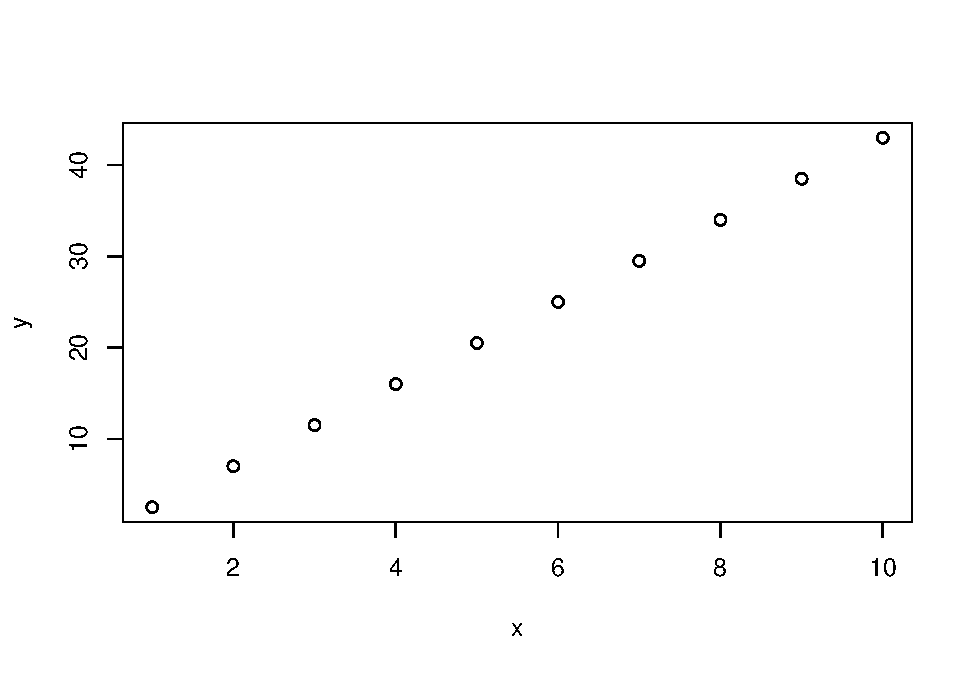
\includegraphics{_main_files/figure-latex/unnamed-chunk-36-1.pdf}

\begin{Shaded}
\begin{Highlighting}[]
\FunctionTok{plot}\NormalTok{(y}\SpecialCharTok{\textasciitilde{}}\NormalTok{x)}
\end{Highlighting}
\end{Shaded}

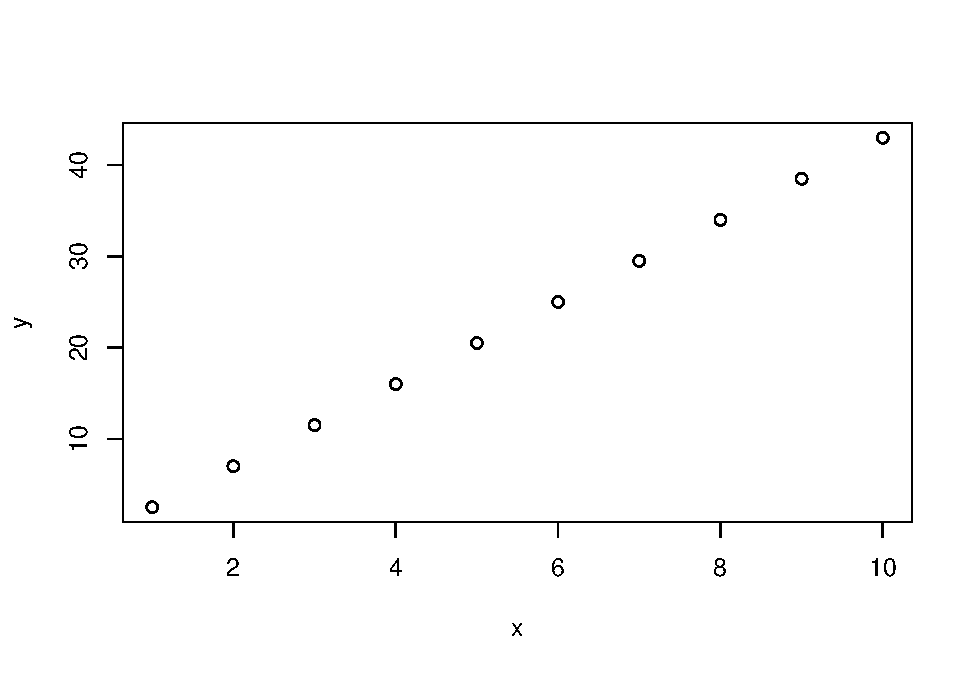
\includegraphics{_main_files/figure-latex/unnamed-chunk-36-2.pdf}

Con type es posible cambiar la disposición del diagrama de dispersión:

\begin{Shaded}
\begin{Highlighting}[]
\FunctionTok{plot}\NormalTok{(x, y, }\AttributeTok{type=}\StringTok{"l"}\NormalTok{)}
\end{Highlighting}
\end{Shaded}

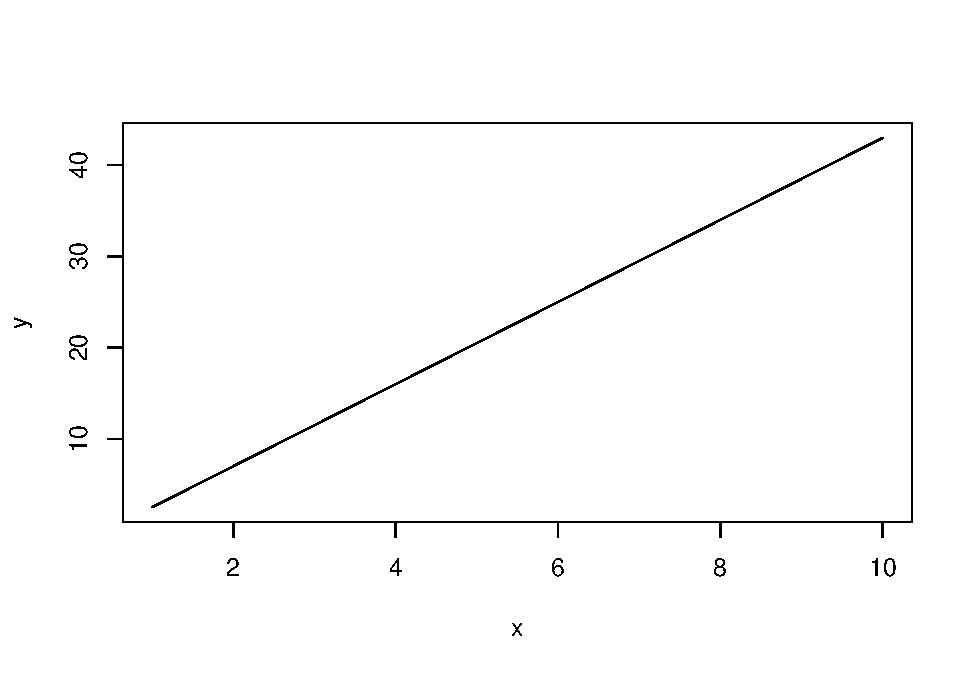
\includegraphics{_main_files/figure-latex/unnamed-chunk-37-1.pdf}

\begin{Shaded}
\begin{Highlighting}[]
\FunctionTok{plot}\NormalTok{(x, y, }\AttributeTok{type=}\StringTok{"b"}\NormalTok{)}
\end{Highlighting}
\end{Shaded}

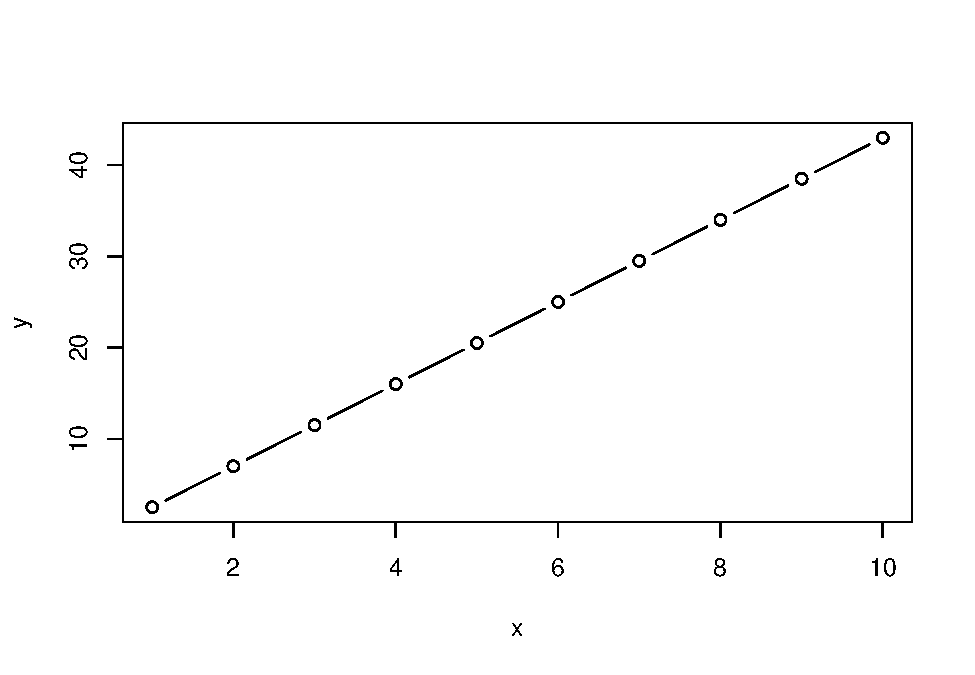
\includegraphics{_main_files/figure-latex/unnamed-chunk-37-2.pdf}

\begin{Shaded}
\begin{Highlighting}[]
\FunctionTok{plot}\NormalTok{(x, y, }\AttributeTok{type=}\StringTok{"c"}\NormalTok{)}
\end{Highlighting}
\end{Shaded}

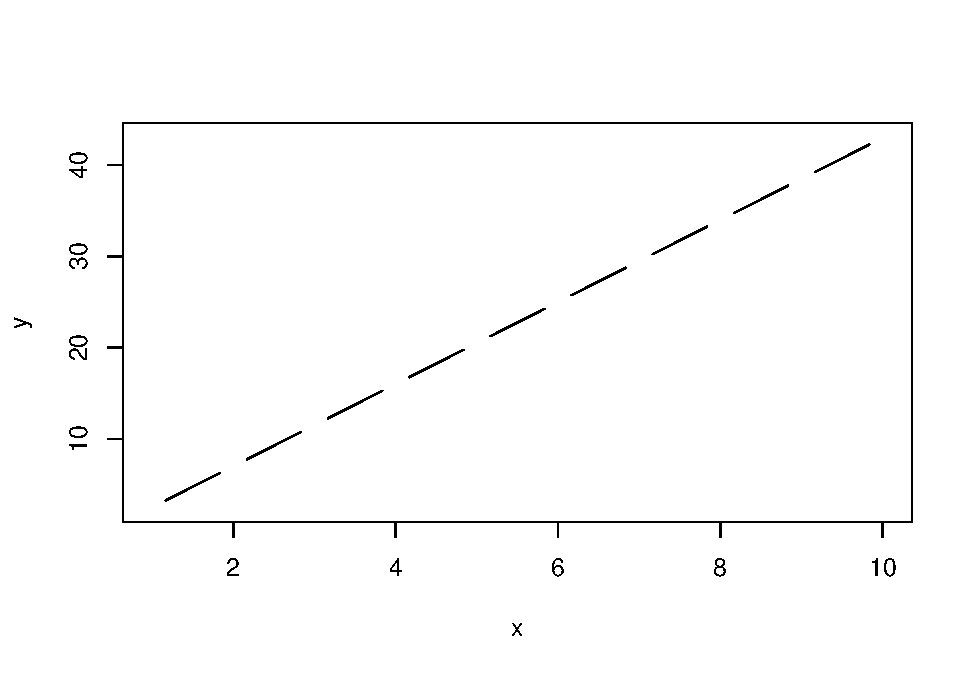
\includegraphics{_main_files/figure-latex/unnamed-chunk-37-3.pdf}

\begin{Shaded}
\begin{Highlighting}[]
\FunctionTok{plot}\NormalTok{(x, y, }\AttributeTok{type=}\StringTok{"o"}\NormalTok{)}
\end{Highlighting}
\end{Shaded}

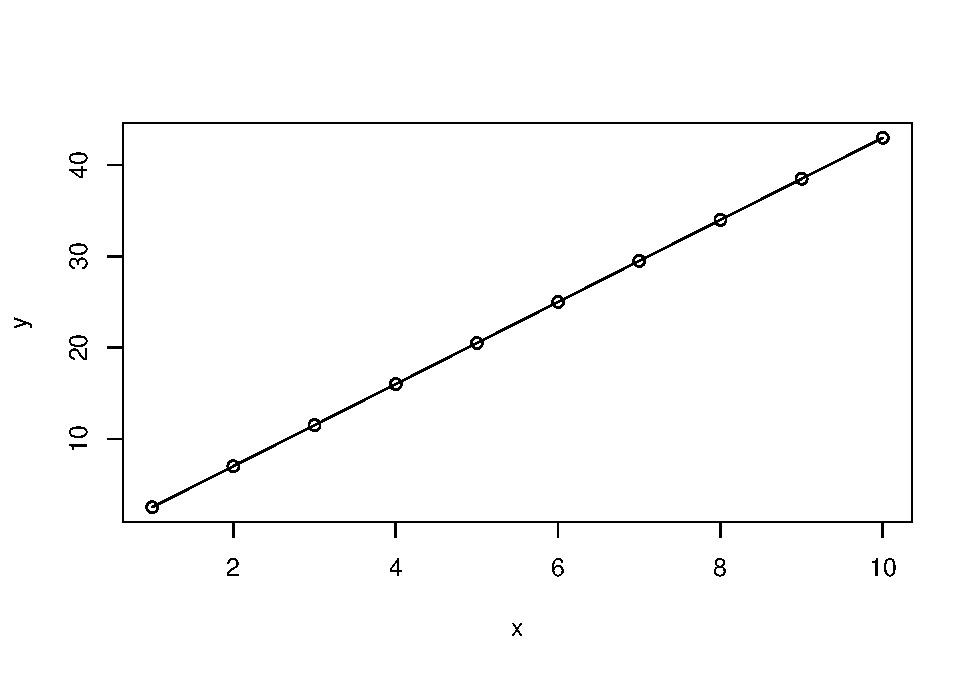
\includegraphics{_main_files/figure-latex/unnamed-chunk-37-4.pdf}

\begin{Shaded}
\begin{Highlighting}[]
\FunctionTok{plot}\NormalTok{(x, y, }\AttributeTok{type=}\StringTok{"h"}\NormalTok{)}
\end{Highlighting}
\end{Shaded}

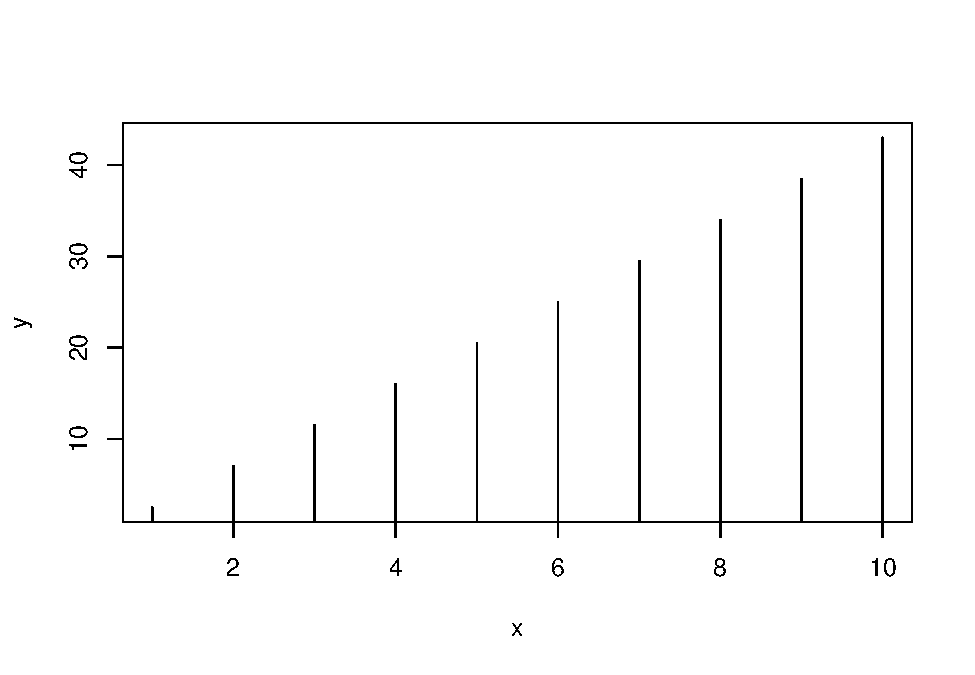
\includegraphics{_main_files/figure-latex/unnamed-chunk-37-5.pdf}

\begin{Shaded}
\begin{Highlighting}[]
\FunctionTok{plot}\NormalTok{(x, y, }\AttributeTok{type=}\StringTok{"n"}\NormalTok{)}
\end{Highlighting}
\end{Shaded}

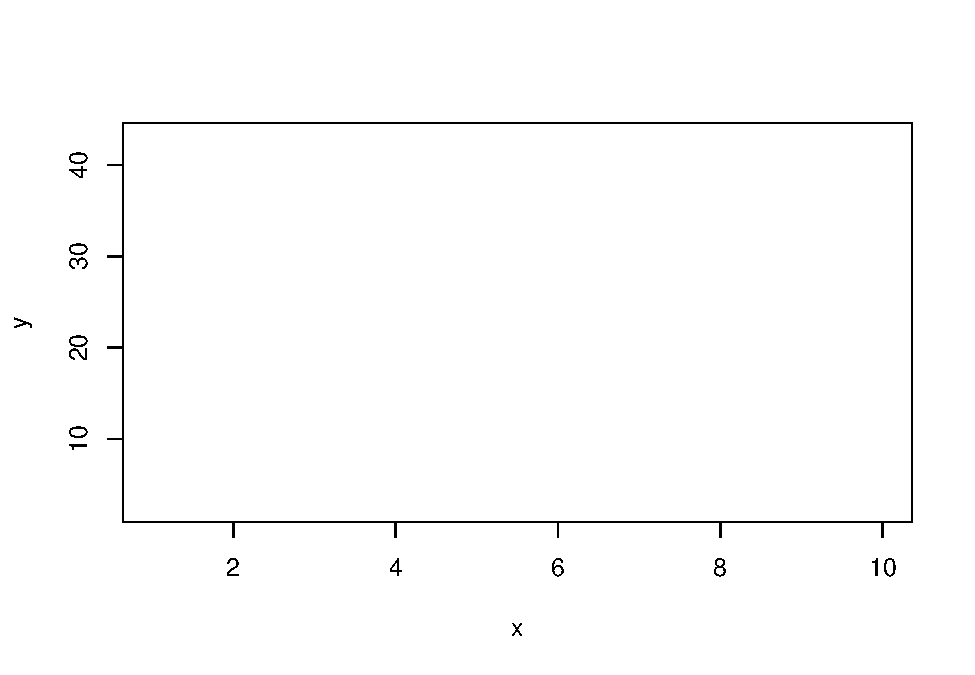
\includegraphics{_main_files/figure-latex/unnamed-chunk-37-6.pdf}

\hypertarget{etiquetas-de-la-gruxe1fica-xlab-ylab-main}{%
\subsection{Etiquetas de la gráfica: xlab, ylab, main}\label{etiquetas-de-la-gruxe1fica-xlab-ylab-main}}

\begin{Shaded}
\begin{Highlighting}[]
\FunctionTok{plot}\NormalTok{(x, y, }\AttributeTok{xlab =} \StringTok{"eje x"}\NormalTok{, }\AttributeTok{ylab =} \StringTok{"eje y"}\NormalTok{, }\AttributeTok{main =} \StringTok{"Titulo del grafico"}\NormalTok{, }\AttributeTok{type =} \StringTok{"n"}\NormalTok{)}
\FunctionTok{points}\NormalTok{(x , y, }\AttributeTok{col =} \StringTok{"red"}\NormalTok{, }\AttributeTok{pch =} \DecValTok{19}\NormalTok{)}
\FunctionTok{lines}\NormalTok{(x, y, }\AttributeTok{col =} \StringTok{"blue"}\NormalTok{)}
\end{Highlighting}
\end{Shaded}

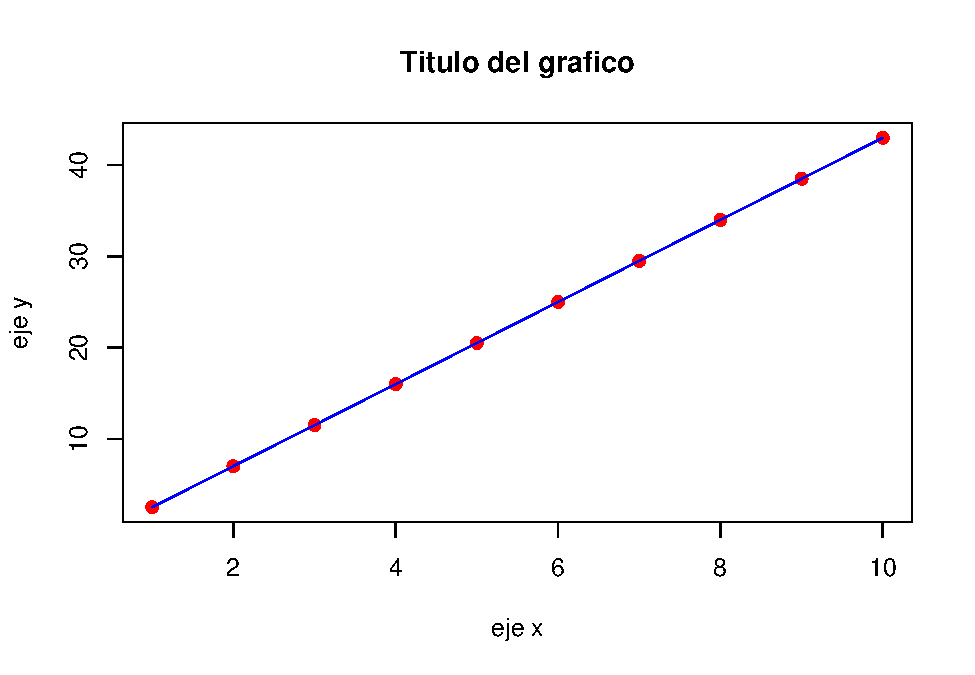
\includegraphics{_main_files/figure-latex/unnamed-chunk-38-1.pdf}

¿Qué ocurre aquí? Por favor explique:

\begin{Shaded}
\begin{Highlighting}[]
\FunctionTok{plot}\NormalTok{(x, y, }\AttributeTok{xlab =} \StringTok{"eje x"}\NormalTok{, }\AttributeTok{ylab =} \StringTok{"eje y"}\NormalTok{, }\AttributeTok{main =} \StringTok{"Titulo del grafico"}\NormalTok{, }\AttributeTok{type =} \StringTok{"n"}\NormalTok{)}
\FunctionTok{points}\NormalTok{(x }\SpecialCharTok{+} \FloatTok{0.5}\NormalTok{, y, }\AttributeTok{col =} \StringTok{"blue"}\NormalTok{, }\AttributeTok{pch =} \DecValTok{15}\NormalTok{, }\AttributeTok{cex =} \FloatTok{5.5}\NormalTok{) }
\end{Highlighting}
\end{Shaded}

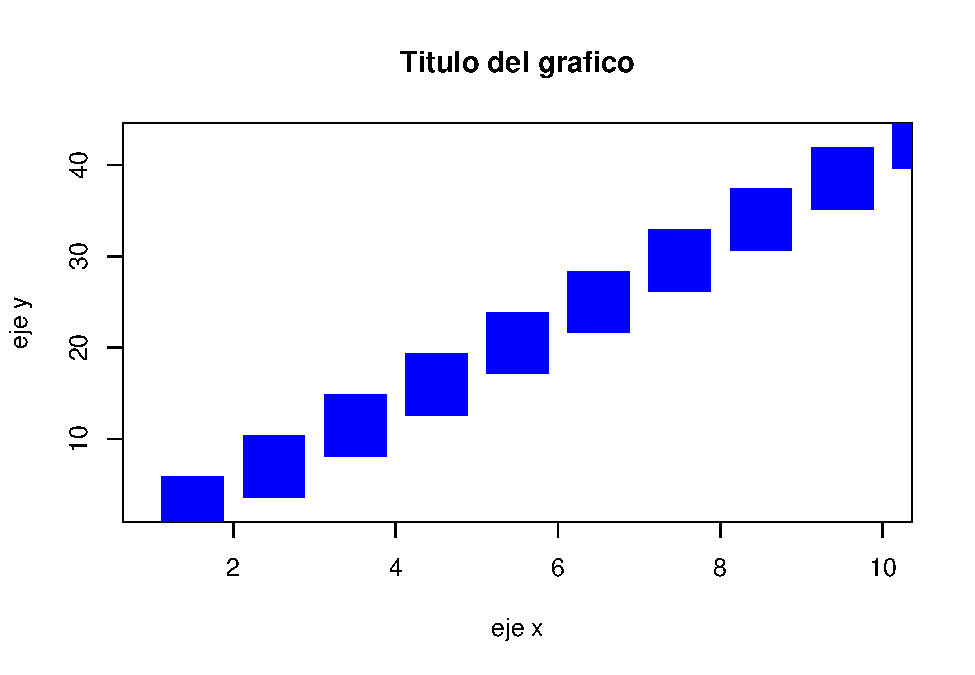
\includegraphics{_main_files/figure-latex/unnamed-chunk-39-1.pdf}

¿Para que son los argumentos ``pch'' y ``cex''?

?points

\textbf{Ejercicios:}

\begin{verbatim}
1. Haga una linea en zigzag con puntos de colores en los puntos de giro

2. Haga una carita (:|)
\end{verbatim}

Más gráficas: \{-\}

\begin{Shaded}
\begin{Highlighting}[]
\NormalTok{x }\OtherTok{\textless{}{-}} \FunctionTok{seq}\NormalTok{(}\AttributeTok{from =} \DecValTok{0}\NormalTok{, }\AttributeTok{to =} \DecValTok{2} \SpecialCharTok{*}\NormalTok{ pi, }\AttributeTok{by =} \FloatTok{0.2}\NormalTok{)}
\NormalTok{y }\OtherTok{\textless{}{-}} \FunctionTok{sin}\NormalTok{(x) }\CommentTok{\# Función seno}
\FunctionTok{plot}\NormalTok{(x, y)}

\NormalTok{z }\OtherTok{\textless{}{-}} \FunctionTok{cos}\NormalTok{(x) }\CommentTok{\#Función coseno}
\FunctionTok{lines}\NormalTok{(x, z)  }\CommentTok{\# Agregamos líneas al grafico anterior }
\FunctionTok{points}\NormalTok{(x, z }\SpecialCharTok{*} \FloatTok{0.5}\NormalTok{, }\AttributeTok{pch =} \DecValTok{16}\NormalTok{) }\CommentTok{\# Agregamos puntos al gráfico anterior }
\end{Highlighting}
\end{Shaded}

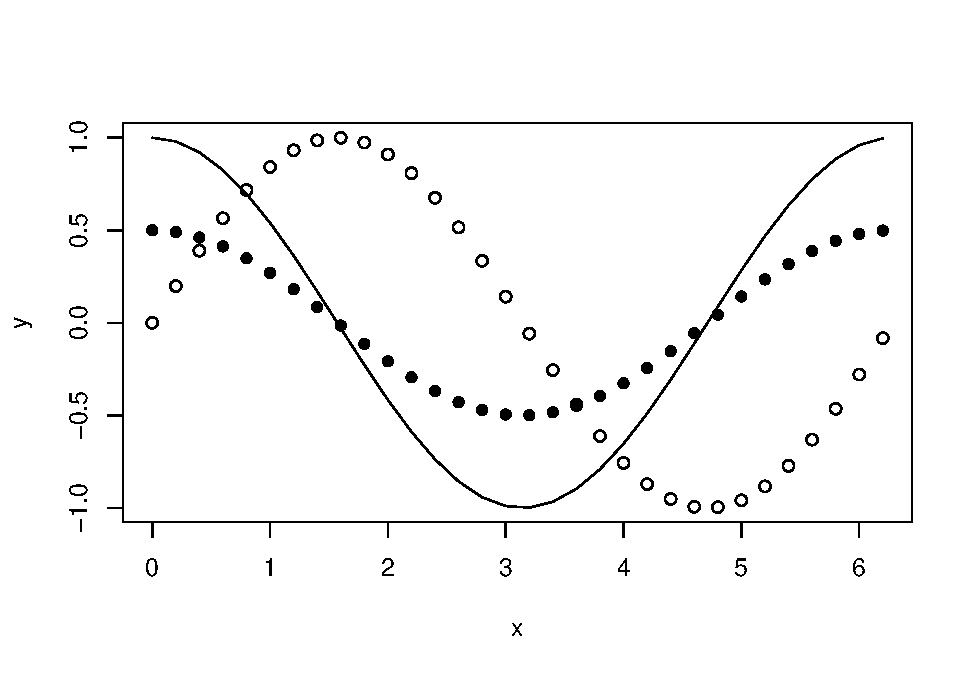
\includegraphics{_main_files/figure-latex/unnamed-chunk-40-1.pdf}

\begin{Shaded}
\begin{Highlighting}[]
\CommentTok{\#De nuevo, eje, etiquetas y título }
\FunctionTok{plot}\NormalTok{(x, y, }\AttributeTok{xlab =} \StringTok{"eje x"}\NormalTok{, }\AttributeTok{type =} \StringTok{"l"}\NormalTok{, }\AttributeTok{ylab =} \StringTok{"eje y"}\NormalTok{, }\AttributeTok{main =} \StringTok{"Curva sinusoidal"}\NormalTok{)}
\end{Highlighting}
\end{Shaded}

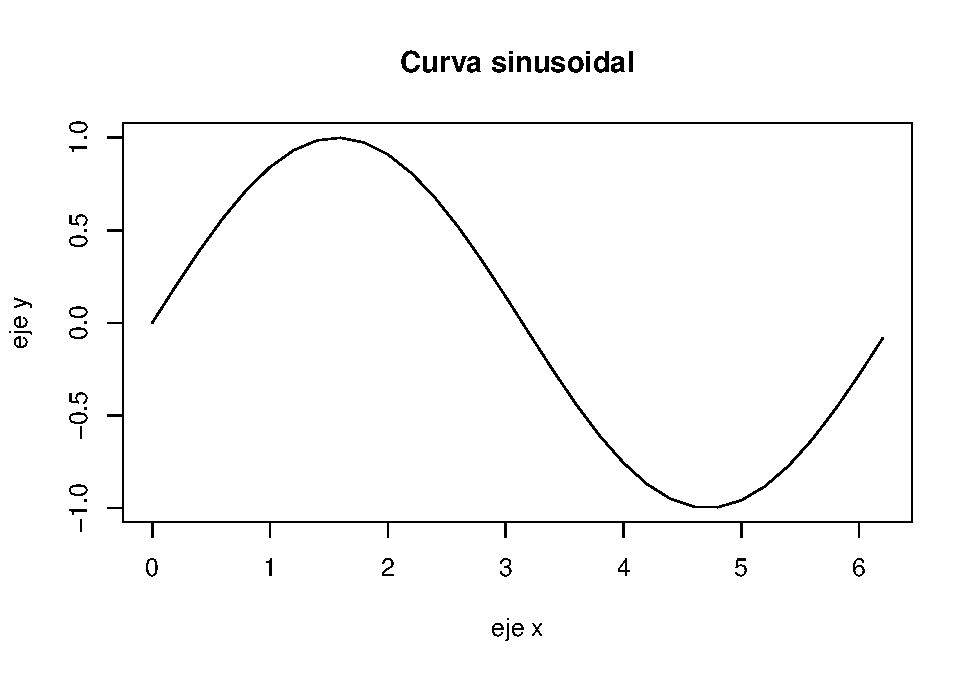
\includegraphics{_main_files/figure-latex/unnamed-chunk-40-2.pdf}

\begin{Shaded}
\begin{Highlighting}[]
\CommentTok{\#Cambiando la extension de los ejes "x" y "y" usando "xlim" y "ylim"}

\FunctionTok{plot}\NormalTok{(x, y, }\AttributeTok{xlab =} \StringTok{"eje x"}\NormalTok{, }\AttributeTok{type =} \StringTok{"l"}\NormalTok{, }\AttributeTok{ylab =} \StringTok{"eje y"}\NormalTok{, }\AttributeTok{main =} \StringTok{"Curva sinusoidal"}\NormalTok{, }
     \AttributeTok{xlim =} \FunctionTok{c}\NormalTok{(}\SpecialCharTok{{-}}\DecValTok{1}\NormalTok{, }\DecValTok{7}\NormalTok{), }\AttributeTok{ylim =} \FunctionTok{c}\NormalTok{(}\SpecialCharTok{{-}}\DecValTok{2}\NormalTok{, }\DecValTok{2}\NormalTok{))}
\end{Highlighting}
\end{Shaded}

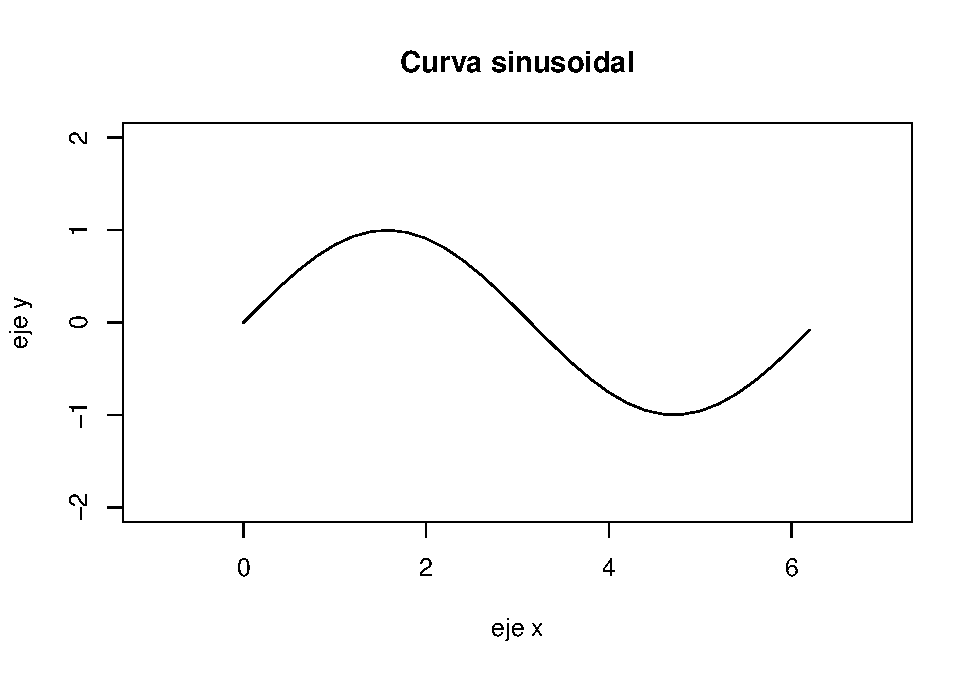
\includegraphics{_main_files/figure-latex/unnamed-chunk-40-3.pdf}

\begin{Shaded}
\begin{Highlighting}[]
\FunctionTok{plot}\NormalTok{(x, y, }\AttributeTok{xlab =} \StringTok{"eje x"}\NormalTok{, }\AttributeTok{type =} \StringTok{"l"}\NormalTok{, }\AttributeTok{ylab =} \StringTok{"eje y"}\NormalTok{, }\AttributeTok{main =} \StringTok{"Curva sinusoidal"}\NormalTok{, }
     \AttributeTok{xlim =} \FunctionTok{c}\NormalTok{(}\DecValTok{2}\NormalTok{, }\DecValTok{4}\NormalTok{), }\AttributeTok{ylim =} \FunctionTok{c}\NormalTok{(}\DecValTok{0}\NormalTok{, }\DecValTok{1}\NormalTok{))}
\end{Highlighting}
\end{Shaded}

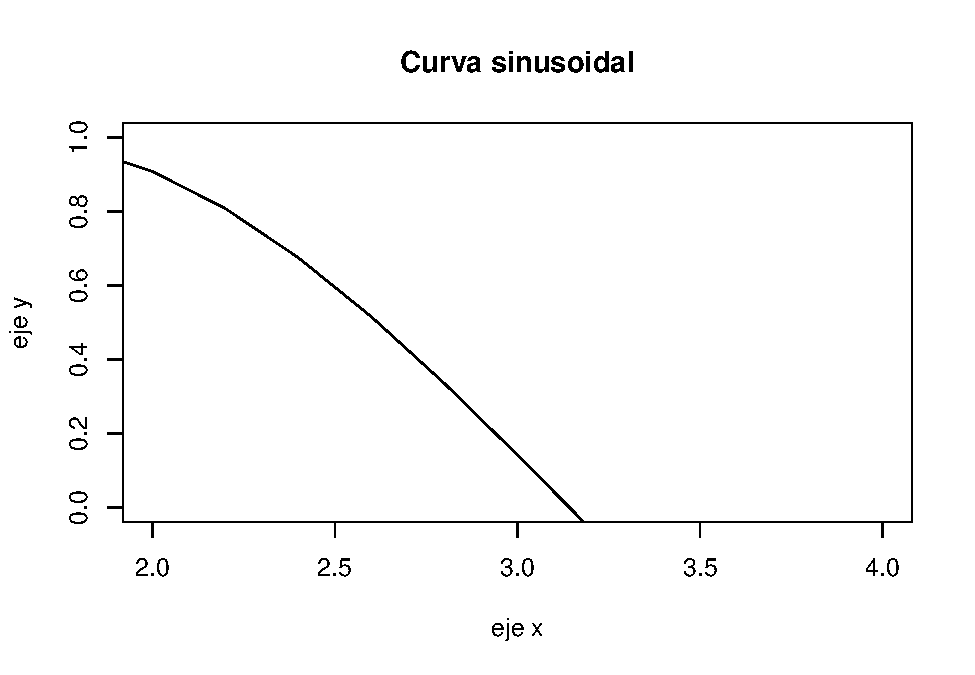
\includegraphics{_main_files/figure-latex/unnamed-chunk-40-4.pdf}

\hypertarget{demostraciuxf3n-de-la-versatilidad-de-la-gruxe1fica}{%
\section{Demostración de la versatilidad de la gráfica}\label{demostraciuxf3n-de-la-versatilidad-de-la-gruxe1fica}}

La representación gráfica en R es muy flexible. Vamos a cambiar mas parametros gráficos:

\begin{itemize}
\tightlist
\item
  `cex': escala de simbolos (tamano)
\end{itemize}

\begin{Shaded}
\begin{Highlighting}[]
\FunctionTok{plot}\NormalTok{(x, y, }\AttributeTok{cex =} \FunctionTok{rep}\NormalTok{(}\DecValTok{1}\SpecialCharTok{:}\DecValTok{8}\NormalTok{, }\AttributeTok{times =} \DecValTok{4}\NormalTok{))}
\end{Highlighting}
\end{Shaded}

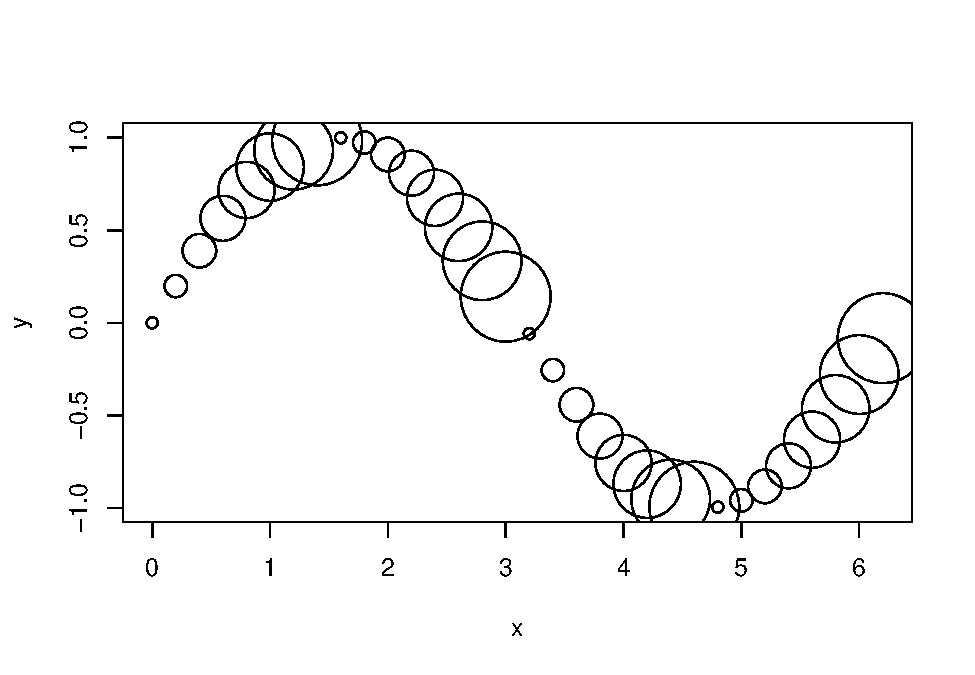
\includegraphics{_main_files/figure-latex/unnamed-chunk-41-1.pdf}

\begin{itemize}
\tightlist
\item
  `pch': cambia el simbolo de los puntos
\end{itemize}

\begin{Shaded}
\begin{Highlighting}[]
\FunctionTok{plot}\NormalTok{(}\DecValTok{1}\SpecialCharTok{:}\DecValTok{25}\NormalTok{, }\DecValTok{1}\SpecialCharTok{:}\DecValTok{25}\NormalTok{, }\AttributeTok{cex =} \DecValTok{2}\NormalTok{, }\AttributeTok{pch =} \DecValTok{1}\SpecialCharTok{:}\DecValTok{25}\NormalTok{)}
\end{Highlighting}
\end{Shaded}

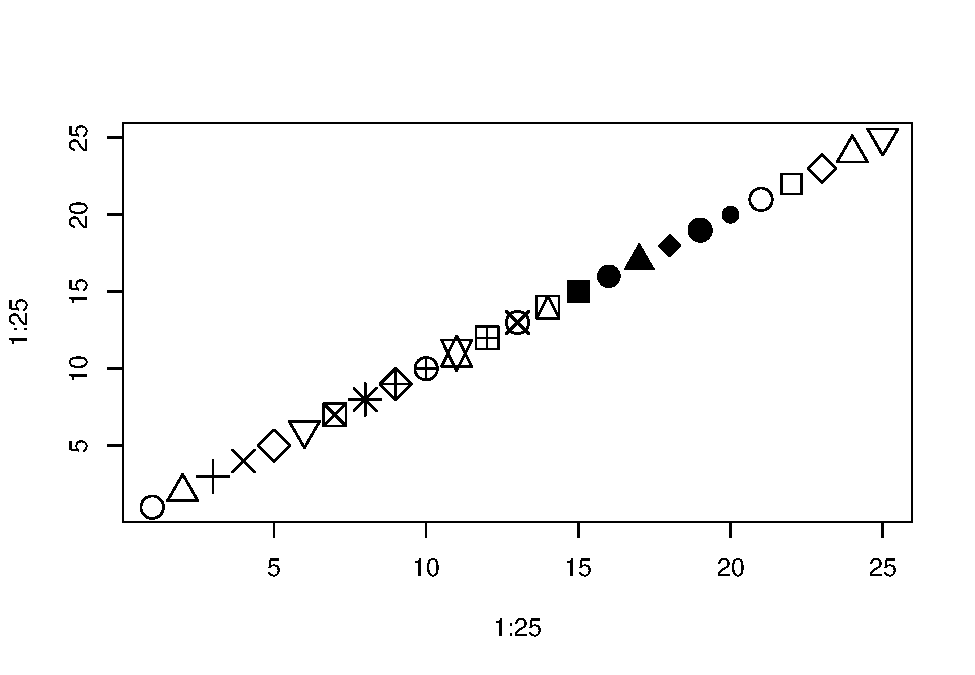
\includegraphics{_main_files/figure-latex/unnamed-chunk-42-1.pdf}

\begin{itemize}
\tightlist
\item
  `col': colores de los puntos. En R estan disponibles mas de 600 colores
\end{itemize}

\begin{Shaded}
\begin{Highlighting}[]
\NormalTok{a }\OtherTok{\textless{}{-}} \FunctionTok{rep}\NormalTok{(}\DecValTok{1}\SpecialCharTok{:}\DecValTok{55}\NormalTok{, }\AttributeTok{times =} \DecValTok{10}\NormalTok{); b }\OtherTok{\textless{}{-}} \FunctionTok{rep}\NormalTok{(}\DecValTok{1}\SpecialCharTok{:}\DecValTok{10}\NormalTok{, }\AttributeTok{each =} \DecValTok{55}\NormalTok{)}
\FunctionTok{plot}\NormalTok{(a, b, }\AttributeTok{pch =} \DecValTok{19}\NormalTok{, }\AttributeTok{cex =} \DecValTok{2}\NormalTok{, }\AttributeTok{col =} \FunctionTok{colors}\NormalTok{()[}\SpecialCharTok{{-}}\FunctionTok{c}\NormalTok{(}\DecValTok{260}\SpecialCharTok{:}\DecValTok{361}\NormalTok{, }\DecValTok{653}\SpecialCharTok{:}\DecValTok{657}\NormalTok{)])}
\end{Highlighting}
\end{Shaded}

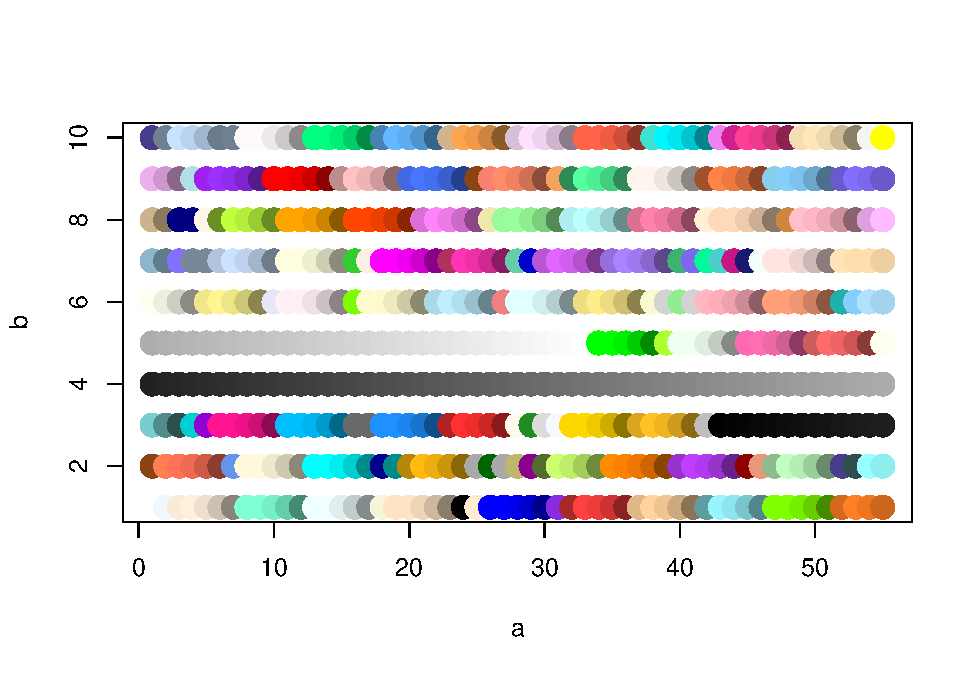
\includegraphics{_main_files/figure-latex/unnamed-chunk-43-1.pdf}

Los gradientes de colores tambien son posibles: ?rainbow

\begin{Shaded}
\begin{Highlighting}[]
\FunctionTok{plot}\NormalTok{(}\DecValTok{1}\SpecialCharTok{:}\DecValTok{100}\NormalTok{, }\DecValTok{1}\SpecialCharTok{:}\DecValTok{100}\NormalTok{, }\AttributeTok{pch =} \DecValTok{19}\NormalTok{, }\AttributeTok{cex =} \DecValTok{3}\NormalTok{, }\AttributeTok{col =} \FunctionTok{rainbow}\NormalTok{(}\DecValTok{100}\NormalTok{))}
\end{Highlighting}
\end{Shaded}

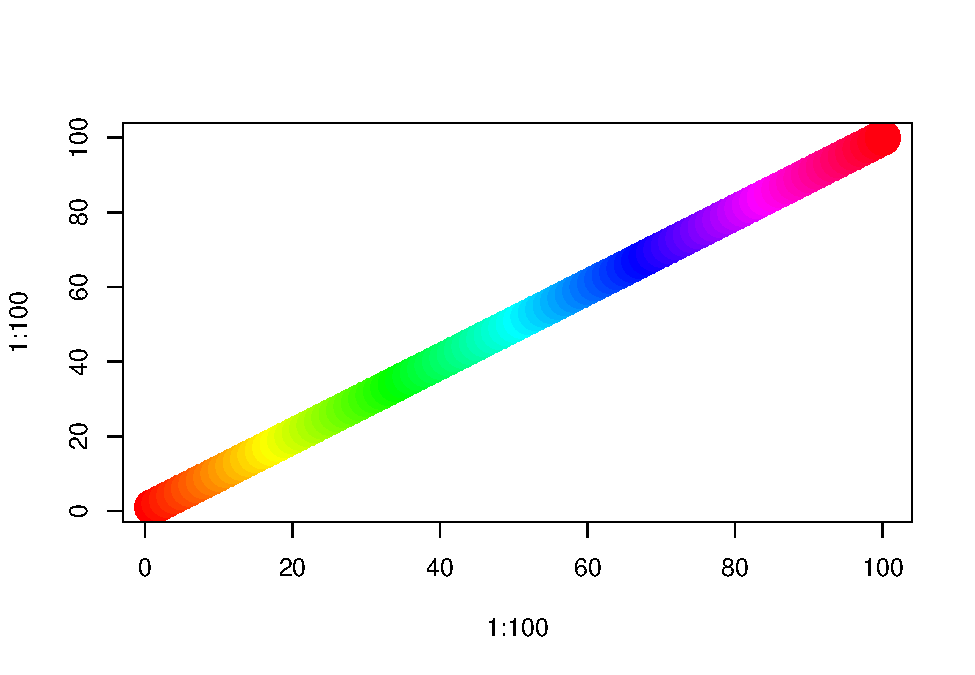
\includegraphics{_main_files/figure-latex/unnamed-chunk-44-1.pdf}

Para los simbolos 21 a 25 de los puntos (ver ?points) puede tener diferentes colores de relleno

\begin{Shaded}
\begin{Highlighting}[]
\FunctionTok{plot}\NormalTok{ (}\DecValTok{1}\SpecialCharTok{:}\DecValTok{25}\NormalTok{, }\AttributeTok{cex=}\DecValTok{2}\NormalTok{, }\AttributeTok{pch=}\DecValTok{1}\SpecialCharTok{:}\DecValTok{25}\NormalTok{, }\AttributeTok{col=}\StringTok{"blue"}\NormalTok{, }\AttributeTok{bg=}\StringTok{"red"}\NormalTok{)}
\end{Highlighting}
\end{Shaded}

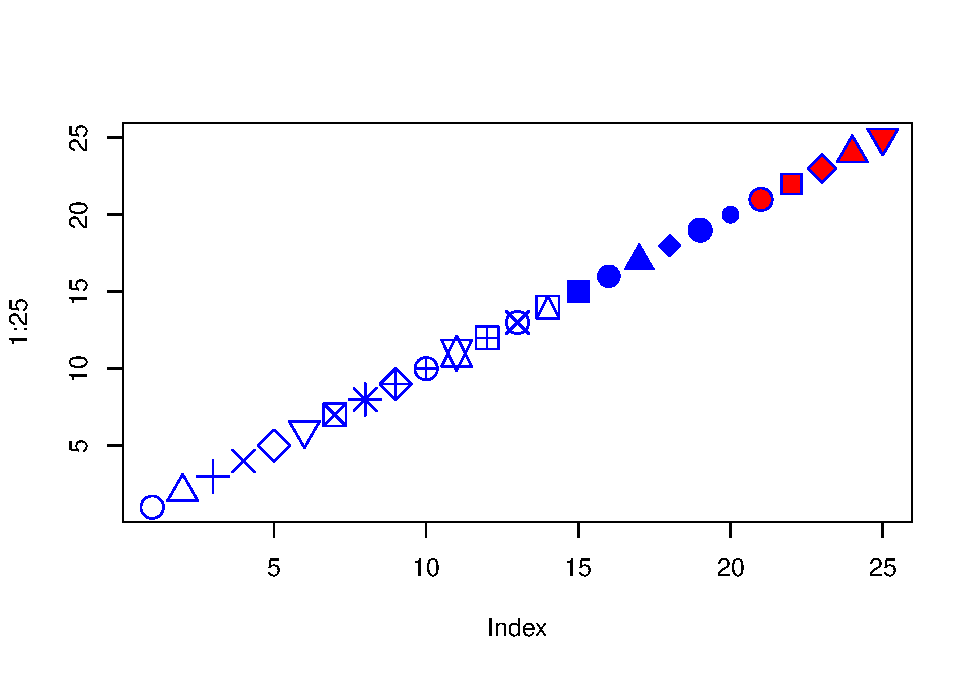
\includegraphics{_main_files/figure-latex/unnamed-chunk-45-1.pdf}

\textbf{Ejercicios:}

\begin{verbatim}
1. Consulte la pagina web de Quick-R para ver ejemplos de diagramas de dispersion (http://www.statmethods.net/graphs/scatterplot.html) y elija uno que explique a sus colegas.
\end{verbatim}

\hypertarget{barras-cajas-e-histogramas}{%
\section{Barras, cajas e histogramas}\label{barras-cajas-e-histogramas}}

Algunas de las gráficas más populares para reportar y explorar datos es mediante las graficas de barras (conteo de observaciones), cajas (estadisticos de nuestros datos) e histogramas (frecuencia de valores)

En R, estas gráficas se realizan meidante las siguientes funciones:

?barplot()
?boxplot()
?hist()

Vamos a explorar estas funciones.

Si queremos ver el número de registros de nuestras variables, podemos hacerlo mediante una gráfica de barras. Para poder graficarlo, necesitamos un vector o matriz que conenga valores numéricos.

\begin{Shaded}
\begin{Highlighting}[]
\NormalTok{x }\OtherTok{\textless{}{-}} \FunctionTok{c}\NormalTok{(}\DecValTok{100}\NormalTok{,}\DecValTok{20}\NormalTok{,}\DecValTok{70}\NormalTok{,}\DecValTok{240}\NormalTok{,}\DecValTok{230}\NormalTok{)}

\FunctionTok{barplot}\NormalTok{(x)}
\end{Highlighting}
\end{Shaded}

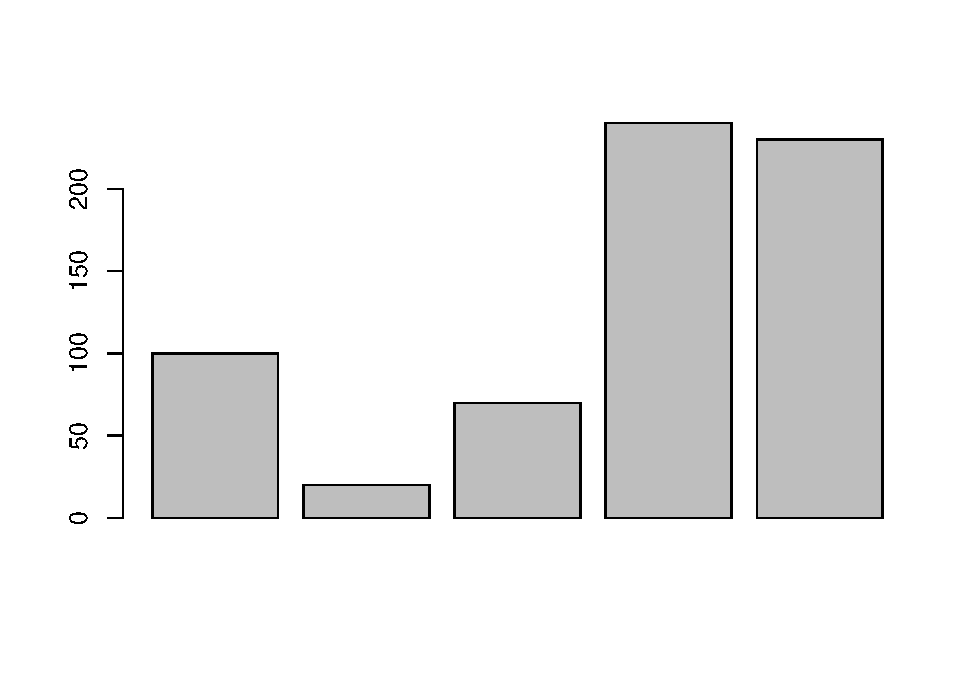
\includegraphics{_main_files/figure-latex/unnamed-chunk-46-1.pdf}

\begin{Shaded}
\begin{Highlighting}[]
\FunctionTok{barplot}\NormalTok{(x, }\AttributeTok{names.arg =} \FunctionTok{c}\NormalTok{(}\StringTok{"x1"}\NormalTok{, }\StringTok{"x2"}\NormalTok{, }\StringTok{"x3"}\NormalTok{, }\StringTok{"x4"}\NormalTok{, }\StringTok{"x5"}\NormalTok{)) }\CommentTok{\#Asignamos nombres a cada barra}
\end{Highlighting}
\end{Shaded}

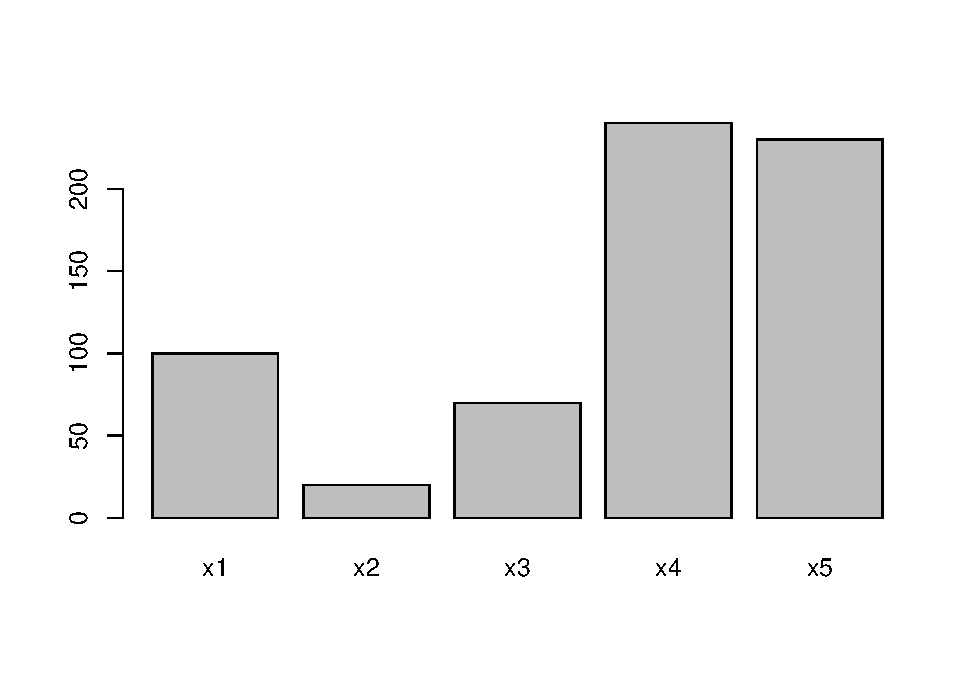
\includegraphics{_main_files/figure-latex/unnamed-chunk-46-2.pdf}

\begin{Shaded}
\begin{Highlighting}[]
\FunctionTok{barplot}\NormalTok{(x, }\AttributeTok{names.arg =} \FunctionTok{c}\NormalTok{(}\StringTok{"x1"}\NormalTok{, }\StringTok{"x2"}\NormalTok{, }\StringTok{"x3"}\NormalTok{, }\StringTok{"x4"}\NormalTok{, }\StringTok{"x5"}\NormalTok{), }\AttributeTok{horiz =} \ConstantTok{TRUE}\NormalTok{) }\CommentTok{\#Podemos invertir los ejes}
\end{Highlighting}
\end{Shaded}

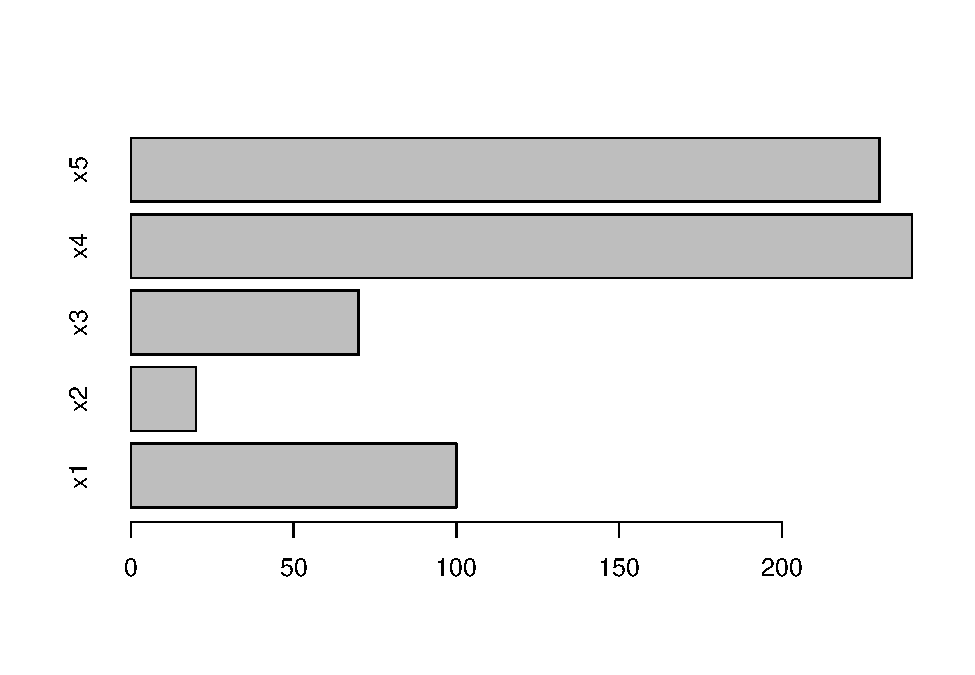
\includegraphics{_main_files/figure-latex/unnamed-chunk-46-3.pdf}

\begin{Shaded}
\begin{Highlighting}[]
\FunctionTok{barplot}\NormalTok{(x, }\AttributeTok{names.arg =} \FunctionTok{c}\NormalTok{(}\StringTok{"x1"}\NormalTok{, }\StringTok{"x2"}\NormalTok{, }\StringTok{"x3"}\NormalTok{, }\StringTok{"x4"}\NormalTok{, }\StringTok{"x5"}\NormalTok{), }\AttributeTok{ylim =} \FunctionTok{c}\NormalTok{(}\DecValTok{0}\NormalTok{,}\DecValTok{100}\NormalTok{)) }\CommentTok{\#Podemos limitar el valor de los ejes}
\end{Highlighting}
\end{Shaded}

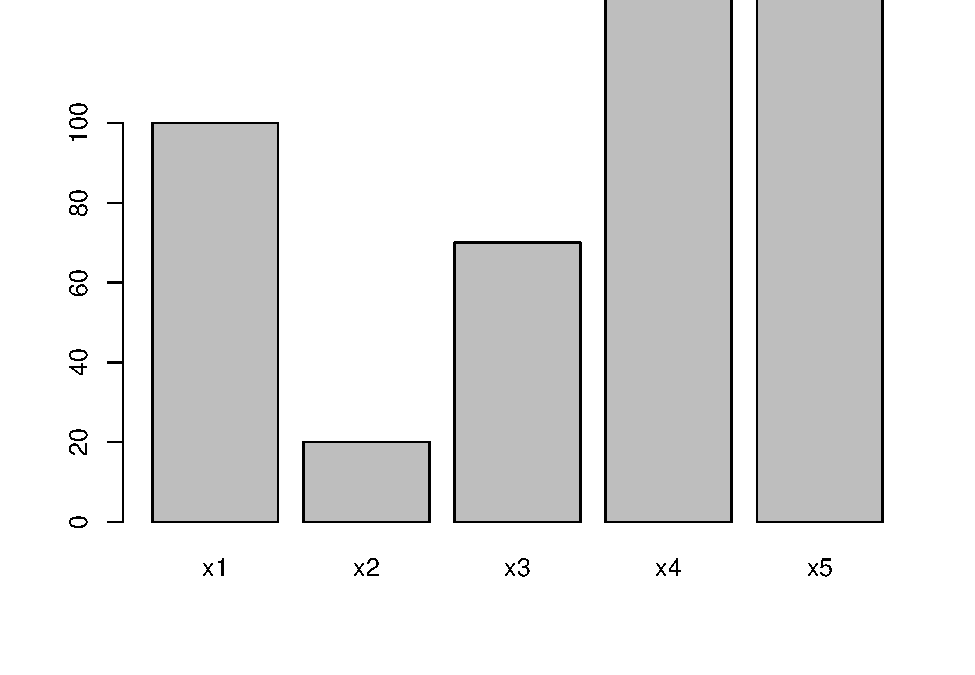
\includegraphics{_main_files/figure-latex/unnamed-chunk-46-4.pdf}

Realice la misma gráfica anterior pero con colores, nombres en los ejes y título.

Mediante boxplot podemos hacer gráficos sencillos que nos muestren datos estadísticos de nuestros datos

\begin{Shaded}
\begin{Highlighting}[]
\FunctionTok{data}\NormalTok{(iris)}
\end{Highlighting}
\end{Shaded}

Cargamos un set de datos predeterminado en R y observamos su contenido.

El set de datos iris se trata de medidas del sépalo y pétalo de distintas especies de plantas.

\begin{Shaded}
\begin{Highlighting}[]
\FunctionTok{boxplot}\NormalTok{(iris}\SpecialCharTok{$}\NormalTok{Sepal.Length) }\CommentTok{\# En este boxplot podemos ver la mediana (linea negra central), los cuatiles 1 y 3 (area gris) y los valores atípicos o outliers (lineas extremas) de los valores de longitud del sepalo de todas las especies }
\end{Highlighting}
\end{Shaded}

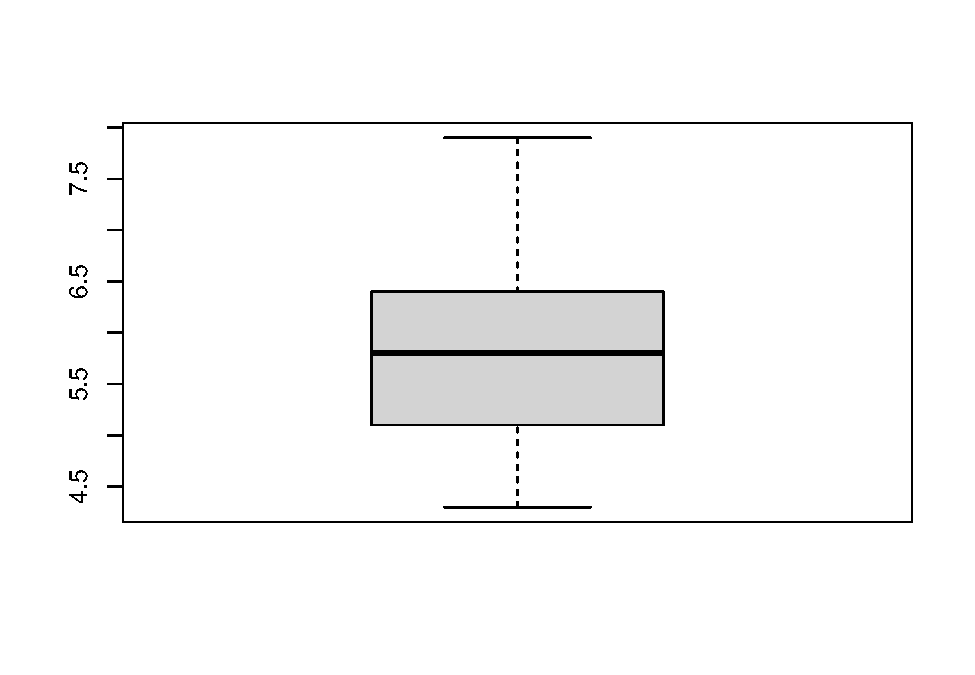
\includegraphics{_main_files/figure-latex/unnamed-chunk-48-1.pdf}

\begin{Shaded}
\begin{Highlighting}[]
\FunctionTok{boxplot}\NormalTok{(Petal.Length }\SpecialCharTok{\textasciitilde{}}\NormalTok{ Species, }\AttributeTok{data =}\NormalTok{ iris) }\CommentTok{\#Podemos graficar los estadisticos para cada grupo usando el simbolo "\textasciitilde{}"}
\end{Highlighting}
\end{Shaded}

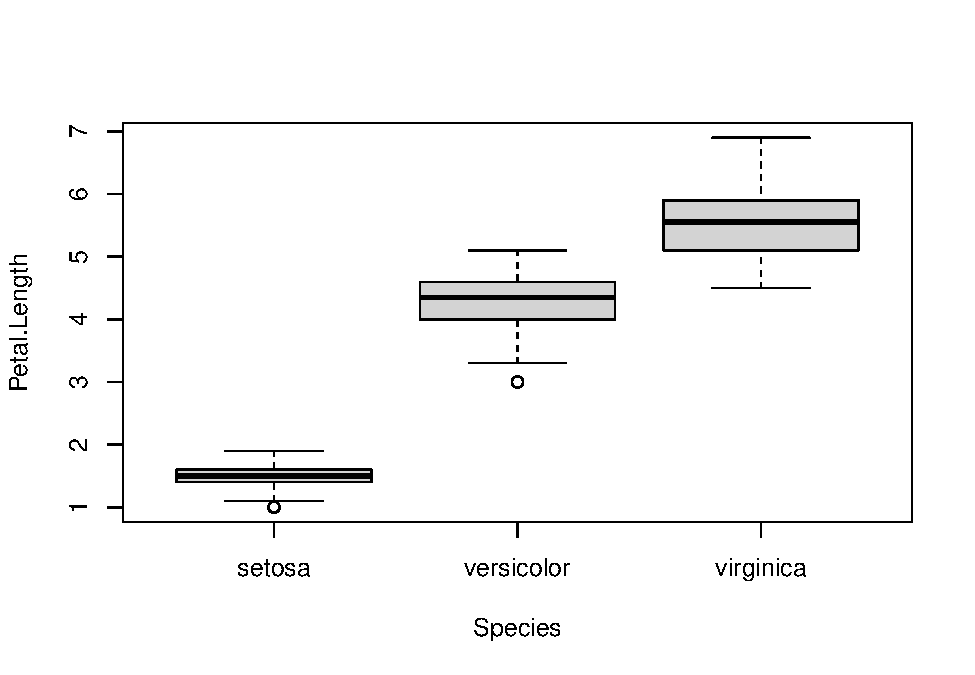
\includegraphics{_main_files/figure-latex/unnamed-chunk-48-2.pdf}

¿Qué pasa si invertimos las variables?

\begin{verbatim}
boxplot(Species ~ Petal.Length, data = iris)
\end{verbatim}

Finalmente, mediante el gráfico de histograma podemos explorar frecuencias de valores.

\begin{Shaded}
\begin{Highlighting}[]
\FunctionTok{hist}\NormalTok{(iris}\SpecialCharTok{$}\NormalTok{Sepal.Length) }\CommentTok{\# En el grafico, el observamos la frecuencia (eje y) y el rango de valores que toma la variable (eje x)}
\end{Highlighting}
\end{Shaded}

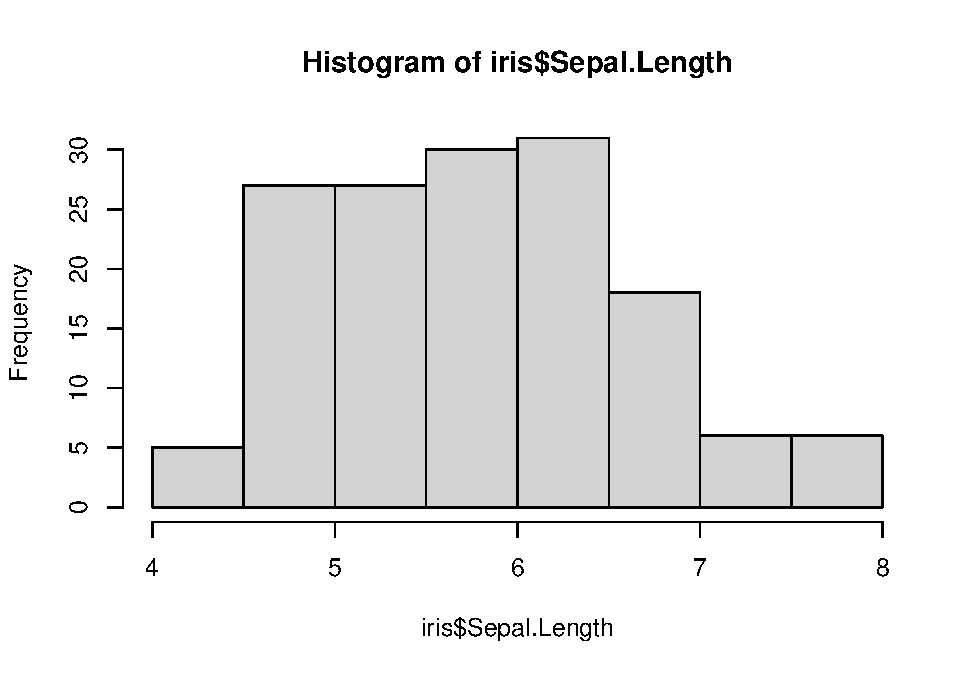
\includegraphics{_main_files/figure-latex/unnamed-chunk-49-1.pdf}

\begin{Shaded}
\begin{Highlighting}[]
\FunctionTok{hist}\NormalTok{(iris}\SpecialCharTok{$}\NormalTok{Petal.Width, }\AttributeTok{col =} \StringTok{"yellow"}\NormalTok{)}
\end{Highlighting}
\end{Shaded}

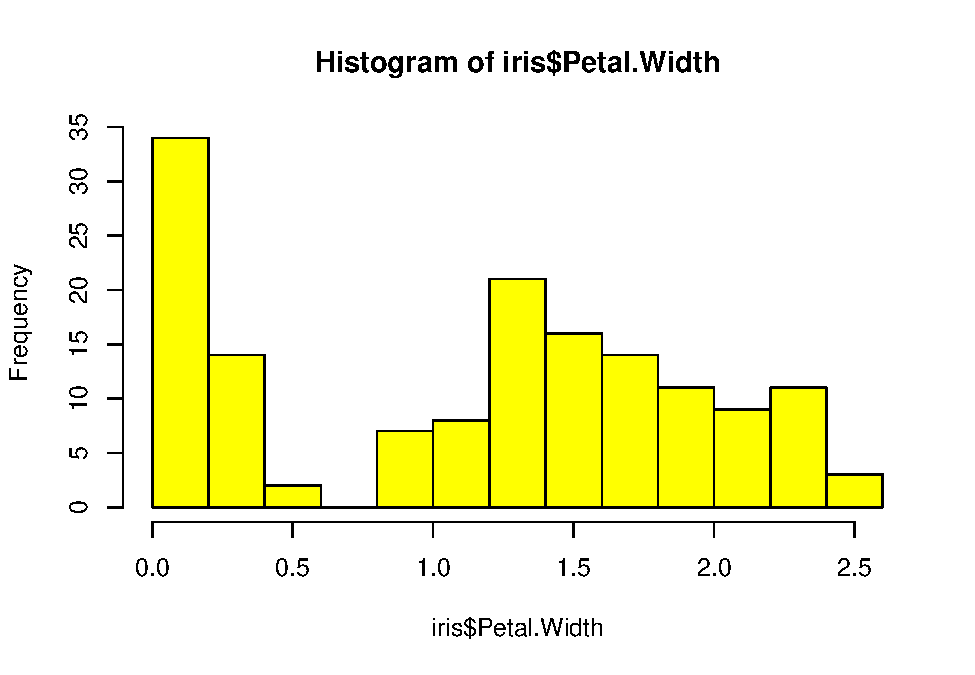
\includegraphics{_main_files/figure-latex/unnamed-chunk-49-2.pdf}

Explore los diferentes argumentos dentro de cada función.

\hypertarget{funciuxf3n-par}{%
\section{Función par()}\label{funciuxf3n-par}}

Mediante la función par() podemos ajustar distintos parametros de nuestra gráfica, asi como mostrar mas de una gráfica al tiempo, colores, texto y muchas otras características

?par

\begin{Shaded}
\begin{Highlighting}[]
\NormalTok{opar }\OtherTok{\textless{}{-}} \FunctionTok{par}\NormalTok{() }\CommentTok{\#Antes de empezar a utilizar par, guardamos la configuración por defecto en un vector para reestablecer su configuracion por defecto}

\FunctionTok{dev.off}\NormalTok{() }\CommentTok{\#O podemos cerrar los plots creados anteriormente para reestablecer la configuración}
\SpecialCharTok{{-}}\NormalTok{ null device }
\SpecialCharTok{{-}}           \DecValTok{1}
\NormalTok{dat\_dias }\OtherTok{\textless{}{-}} \FunctionTok{data.frame}\NormalTok{(}
  \AttributeTok{dias =} \FunctionTok{c}\NormalTok{(}\StringTok{"lunes"}\NormalTok{, }\StringTok{"martes"}\NormalTok{, }\StringTok{"miercoles"}\NormalTok{, }\StringTok{"jueves"}\NormalTok{, }\StringTok{"viernes"}\NormalTok{), }
  \AttributeTok{ganancias =} \FunctionTok{c}\NormalTok{(}\DecValTok{20}\NormalTok{,}\DecValTok{35}\NormalTok{,}\DecValTok{40}\NormalTok{,}\DecValTok{10}\NormalTok{,}\DecValTok{27}\NormalTok{))}
\end{Highlighting}
\end{Shaded}

Realizaremos dos gráficas al tiempo mediante el argumento mfrow

\begin{Shaded}
\begin{Highlighting}[]
\FunctionTok{par}\NormalTok{(}\AttributeTok{mfrow =} \FunctionTok{c}\NormalTok{(}\DecValTok{1}\NormalTok{,}\DecValTok{2}\NormalTok{))}
\FunctionTok{barplot}\NormalTok{(dat\_dias}\SpecialCharTok{$}\NormalTok{ganancias, }\AttributeTok{main =} \StringTok{"Barras"}\NormalTok{, }\AttributeTok{names.arg =}\NormalTok{ dat\_dias}\SpecialCharTok{$}\NormalTok{dias)}
\FunctionTok{pie}\NormalTok{(dat\_dias}\SpecialCharTok{$}\NormalTok{ganancias, }\AttributeTok{labels =}\NormalTok{ dat\_dias}\SpecialCharTok{$}\NormalTok{dias, }\AttributeTok{main =} \StringTok{"Torta"}\NormalTok{, }\AttributeTok{clockwise =}\NormalTok{ T)}
\end{Highlighting}
\end{Shaded}

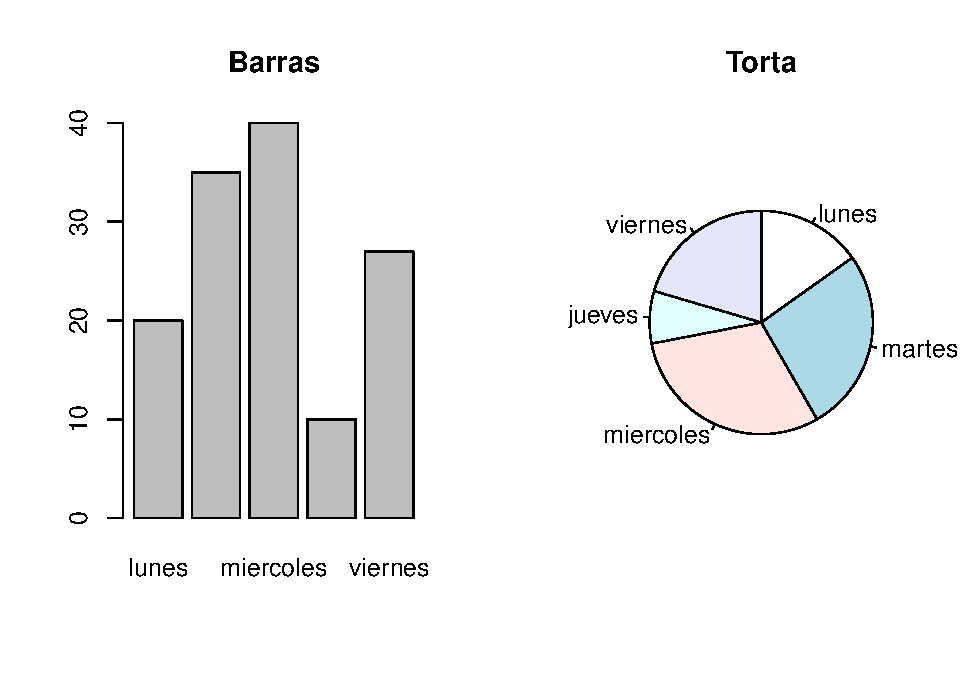
\includegraphics{_main_files/figure-latex/unnamed-chunk-51-1.pdf}

Utilice el argumento bg para cambiar el color de fondo del siguiente plot

\begin{Shaded}
\begin{Highlighting}[]
\FunctionTok{plot}\NormalTok{(}\AttributeTok{x =} \FunctionTok{c}\NormalTok{(}\DecValTok{1}\SpecialCharTok{:}\DecValTok{10}\NormalTok{), }\AttributeTok{y =} \FunctionTok{c}\NormalTok{(}\DecValTok{11}\SpecialCharTok{:}\DecValTok{20}\NormalTok{))}

\FunctionTok{par}\NormalTok{(}\AttributeTok{mfrow =} \FunctionTok{c}\NormalTok{(}\DecValTok{1}\NormalTok{,}\DecValTok{1}\NormalTok{), }\AttributeTok{bg =} \StringTok{"green"}\NormalTok{)}
\FunctionTok{plot}\NormalTok{(}\AttributeTok{x =} \FunctionTok{c}\NormalTok{(}\DecValTok{1}\SpecialCharTok{:}\DecValTok{10}\NormalTok{), }\AttributeTok{y =} \FunctionTok{c}\NormalTok{(}\DecValTok{11}\SpecialCharTok{:}\DecValTok{20}\NormalTok{))}
\end{Highlighting}
\end{Shaded}

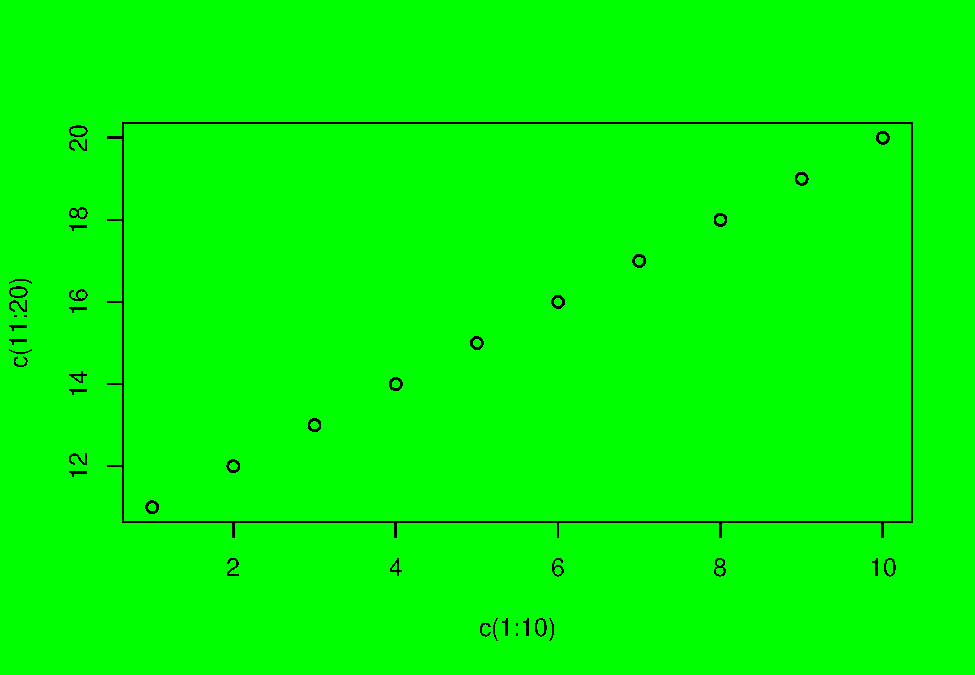
\includegraphics{_main_files/figure-latex/unnamed-chunk-52-1.pdf}

Mediante bty podemos cambiar la forma de la caja del plot:

\begin{Shaded}
\begin{Highlighting}[]
\FunctionTok{par}\NormalTok{(}\AttributeTok{mfrow =} \FunctionTok{c}\NormalTok{(}\DecValTok{1}\NormalTok{,}\DecValTok{1}\NormalTok{), }\AttributeTok{bg =} \StringTok{"white"}\NormalTok{, }\AttributeTok{bty =} \StringTok{"l"}\NormalTok{) }\CommentTok{\#Pruebe cambiando "l" por o,7,c,u,],n}
\FunctionTok{plot}\NormalTok{(}\AttributeTok{x =} \FunctionTok{c}\NormalTok{(}\DecValTok{1}\SpecialCharTok{:}\DecValTok{10}\NormalTok{), }\AttributeTok{y =} \FunctionTok{c}\NormalTok{(}\DecValTok{11}\SpecialCharTok{:}\DecValTok{20}\NormalTok{))}
\end{Highlighting}
\end{Shaded}

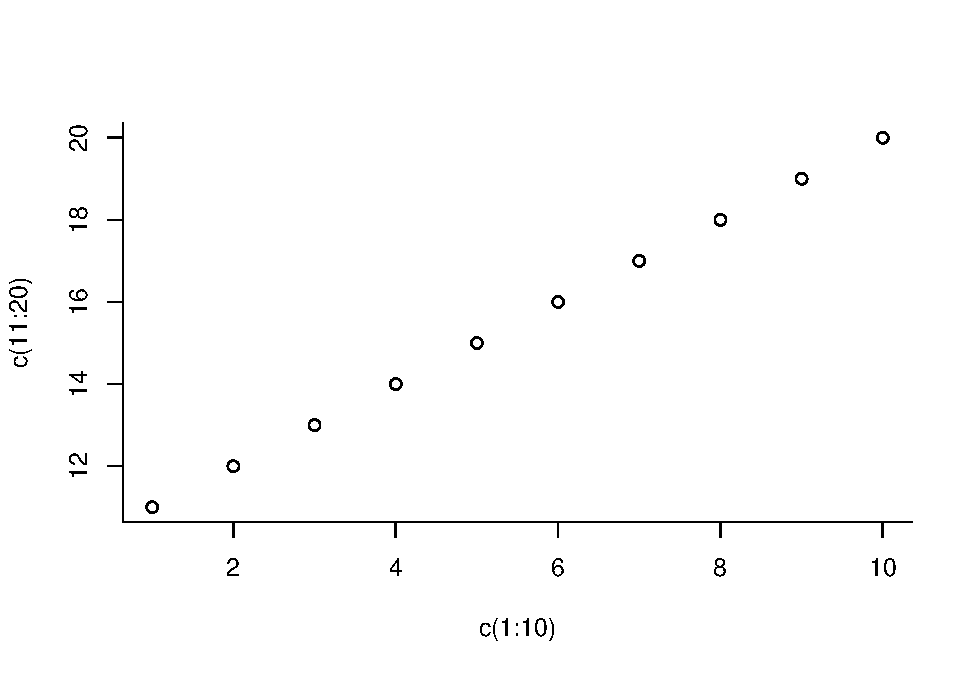
\includegraphics{_main_files/figure-latex/unnamed-chunk-53-1.pdf}

Podemos agregar colores a los diferentes elementos del gráfico

\begin{Shaded}
\begin{Highlighting}[]
\FunctionTok{par}\NormalTok{(}\AttributeTok{mfrow =} \FunctionTok{c}\NormalTok{(}\DecValTok{1}\NormalTok{,}\DecValTok{1}\NormalTok{), }\AttributeTok{bg =} \StringTok{"white"}\NormalTok{, }\AttributeTok{col.axis =} \StringTok{"blue"}\NormalTok{, }\AttributeTok{col.lab =} \StringTok{"green"}\NormalTok{, }\AttributeTok{col.main =} \StringTok{"red"}\NormalTok{, }\AttributeTok{fg =} \StringTok{"yellow"}\NormalTok{) }
\FunctionTok{plot}\NormalTok{(}\AttributeTok{x =} \FunctionTok{c}\NormalTok{(}\DecValTok{1}\SpecialCharTok{:}\DecValTok{10}\NormalTok{), }\AttributeTok{y =} \FunctionTok{c}\NormalTok{(}\DecValTok{11}\SpecialCharTok{:}\DecValTok{20}\NormalTok{), }\AttributeTok{main =} \StringTok{"Dispersion"}\NormalTok{)}
\end{Highlighting}
\end{Shaded}

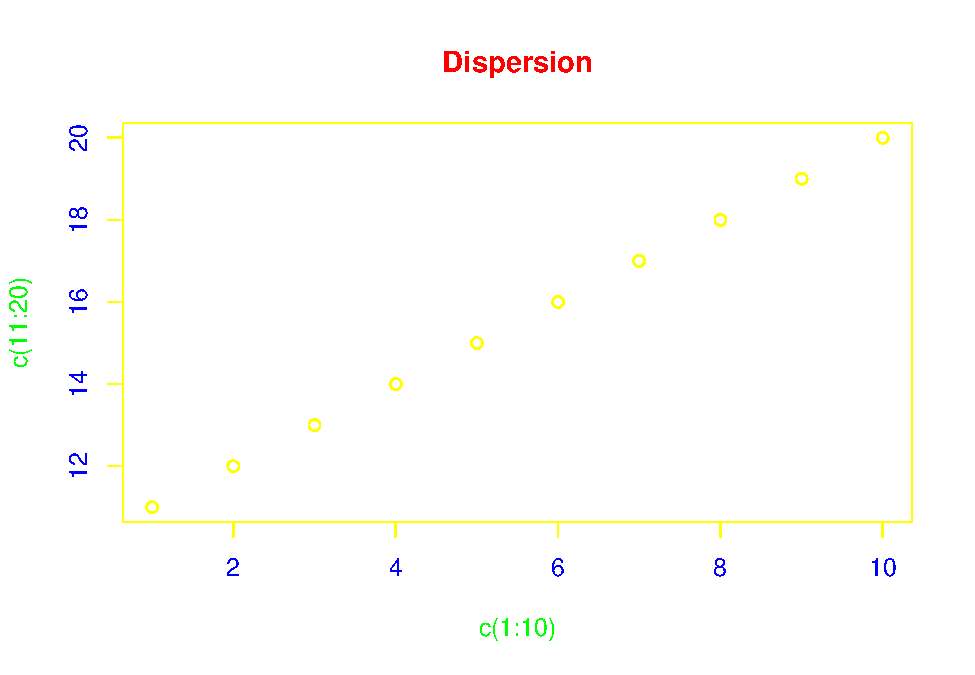
\includegraphics{_main_files/figure-latex/unnamed-chunk-54-1.pdf}

Para cambiar la fuente del texto:

\begin{itemize}
\tightlist
\item
  font.axis = valor numérico
\item
  font.lab
\item
  font.main
\item
  font.sub
\end{itemize}

Explore los siguientes argumentos disponibles en par(), explique su función y utilícelas en una gráfica

\begin{itemize}
\tightlist
\item
  las
\item
  lty
\item
  lwd
\item
  fig
\item
  mai
\item
  pin
\item
  new
\end{itemize}

\begin{Shaded}
\begin{Highlighting}[]
\FunctionTok{par}\NormalTok{(}\AttributeTok{mfrow =} \FunctionTok{c}\NormalTok{(}\DecValTok{1}\NormalTok{,}\DecValTok{1}\NormalTok{), }\AttributeTok{bg =} \StringTok{"white"}\NormalTok{, }\AttributeTok{las =} \DecValTok{3}\NormalTok{, }\AttributeTok{lty =} \DecValTok{3}\NormalTok{, }\AttributeTok{lwd =} \DecValTok{5}\NormalTok{, }\AttributeTok{pin =} \FunctionTok{c}\NormalTok{(}\DecValTok{1}\NormalTok{,}\DecValTok{2}\NormalTok{)) }
\FunctionTok{plot}\NormalTok{(}\AttributeTok{x =} \FunctionTok{c}\NormalTok{(}\DecValTok{1}\SpecialCharTok{:}\DecValTok{10}\NormalTok{), }\AttributeTok{y =} \FunctionTok{c}\NormalTok{(}\DecValTok{11}\SpecialCharTok{:}\DecValTok{20}\NormalTok{), }\AttributeTok{main =} \StringTok{"Dispersión"}\NormalTok{)}
\end{Highlighting}
\end{Shaded}

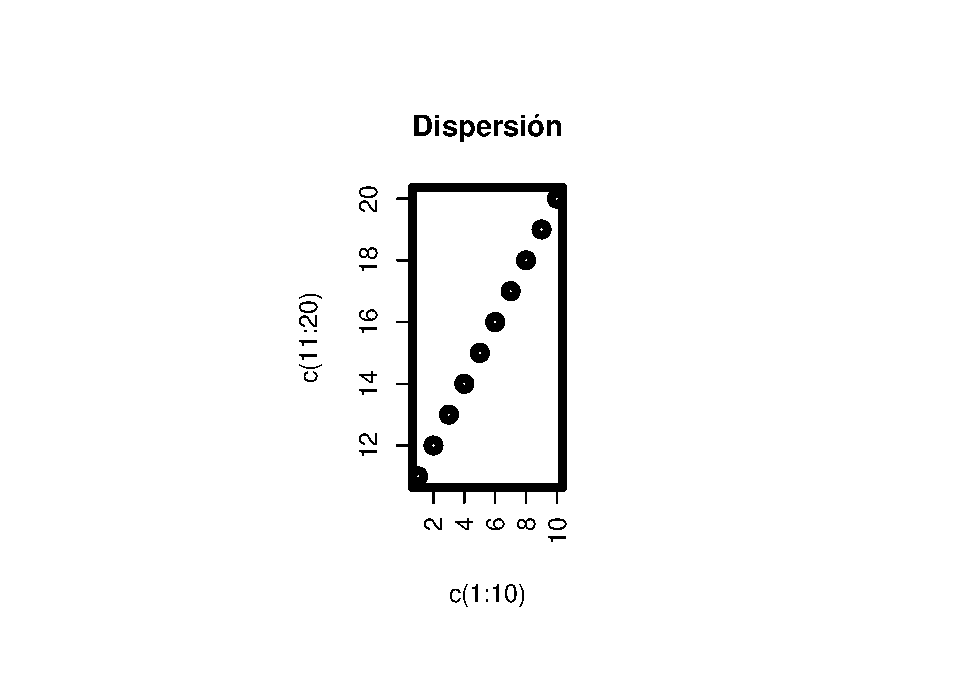
\includegraphics{_main_files/figure-latex/unnamed-chunk-55-1.pdf}

\hypertarget{gruxe1ficos-compuestos}{%
\subsection{Gráficos compuestos}\label{gruxe1ficos-compuestos}}

Usando algunas de las funciones anteriores, podemos ajustar varias figuras en un plot

\begin{Shaded}
\begin{Highlighting}[]
\NormalTok{datos\_aleatorios }\OtherTok{\textless{}{-}} \FunctionTok{runif}\NormalTok{(}\DecValTok{100}\NormalTok{)}

\FunctionTok{par}\NormalTok{(}\AttributeTok{cex=}\FloatTok{0.7}\NormalTok{, }\AttributeTok{mai=}\FunctionTok{c}\NormalTok{(}\FloatTok{0.1}\NormalTok{,}\FloatTok{0.1}\NormalTok{,}\FloatTok{0.2}\NormalTok{,}\FloatTok{0.1}\NormalTok{), }\AttributeTok{fig=}\FunctionTok{c}\NormalTok{(}\FloatTok{0.1}\NormalTok{,}\FloatTok{0.7}\NormalTok{,}\FloatTok{0.3}\NormalTok{,}\FloatTok{0.9}\NormalTok{))}
\FunctionTok{hist}\NormalTok{(datos\_aleatorios) }\CommentTok{\# Configuramos el tamaño de nuestro histograma y lo graficamos}

\FunctionTok{par}\NormalTok{(}\AttributeTok{fig=}\FunctionTok{c}\NormalTok{(}\FloatTok{0.8}\NormalTok{,}\DecValTok{1}\NormalTok{,}\DecValTok{0}\NormalTok{,}\DecValTok{1}\NormalTok{), }\AttributeTok{new=}\ConstantTok{TRUE}\NormalTok{) }\CommentTok{\# Configuramos la posición de un boxplot y agregamos new para que no limpie el gráfico anterior}
\FunctionTok{boxplot}\NormalTok{(datos\_aleatorios)}

\FunctionTok{par}\NormalTok{(}\AttributeTok{fig=}\FunctionTok{c}\NormalTok{(}\FloatTok{0.1}\NormalTok{,}\FloatTok{0.67}\NormalTok{,}\FloatTok{0.1}\NormalTok{,}\FloatTok{0.25}\NormalTok{), }\AttributeTok{new=}\ConstantTok{TRUE}\NormalTok{)}
\FunctionTok{plot}\NormalTok{(}\AttributeTok{x =}\NormalTok{ datos\_aleatorios, }\AttributeTok{y =}\NormalTok{ datos\_aleatorios }\SpecialCharTok{+} \DecValTok{10}\NormalTok{) }\CommentTok{\# Y añadimos un gráfico de dispersion de otro set de datos}
\end{Highlighting}
\end{Shaded}

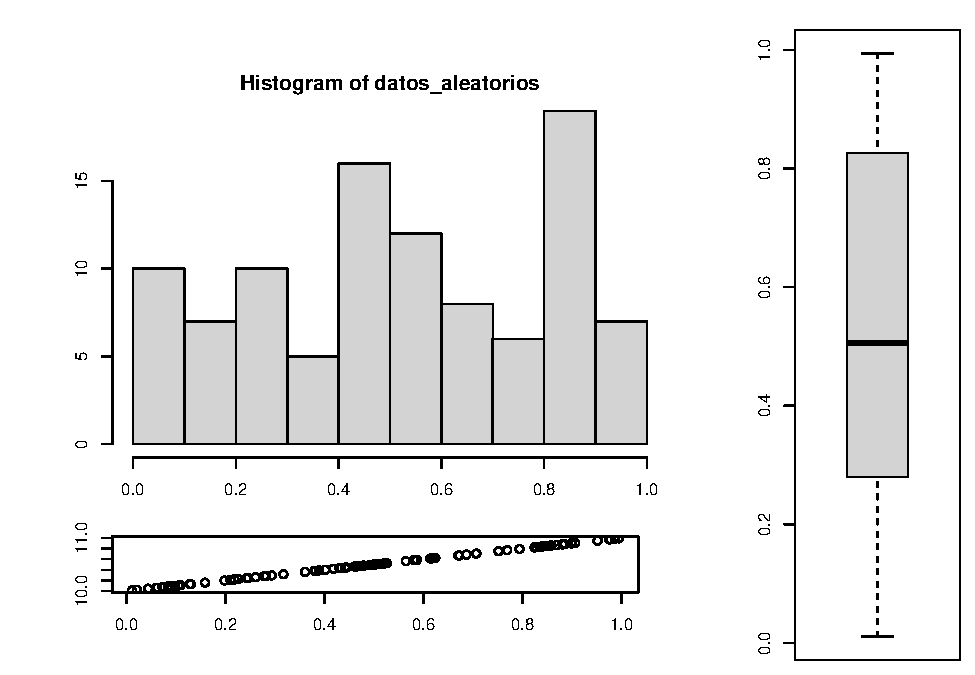
\includegraphics{_main_files/figure-latex/unnamed-chunk-56-1.pdf}

  \bibliography{book.bib}

\end{document}
